% Полезные ссылки:
% * https://habrahabr.ru/post/144648/ - Диплом бакалавра в LaTeX, или ДСТУ 3008-95 в 150 строк
% * http://dkhramov.dp.ua/Comp/NIRReportDSTU300895 - Оформление отчета о НИР в LaTeX
% * http://dkhramov.dp.ua/index.php?n=Comp.CyrillicInListingsTex - Оформление исходного кода в документах LaTeX
% * http://mydebianblog.blogspot.ru/2012/12/latex.html - Как оформить исходный код программ в LaTeX без адских страданий
% * http://aakinshin.blogspot.ru/2014/01/latex-minted.html -  minted: Оформляем исходный код в LaTeX
% * http://s.arboreus.com/2008/12/russian-thesis-in-latex.html - советы: Диссертация в LaTeX

\documentclass[a4paper,12pt]{article}

% Русский язык (LaTeX)
\usepackage[T1,T2A]{fontenc}
\usepackage[utf8]{inputenc}
\usepackage[english,russian]{babel}

% Отступ у первого абзаца
\usepackage[indentfirst]{titlesec}

% Возможность сделать 14-й шрифт
\usepackage{extsizes}
\usepackage{anyfontsize}

% Междустрочный интервал
%\linespread{1.35}
\usepackage[nodisplayskipstretch]{setspace}
\onehalfspacing
% Нет интервала между элементами списков
\usepackage{enumitem}
\setlist{nosep}
% Отступы в списках
%\setitemize[0]{leftmargin=0pt, itemindent=35pt}
\setitemize[0]{leftmargin=1.5cm, itemindent=0cm}
\setenumerate[0]{leftmargin=1.5cm, itemindent=0cm}

% Интервал между абзацами
\setlength{\parskip}{6pt}

% Поля страницы
\usepackage[left=3cm,top=2cm,right=1cm,bottom=2cm]{geometry}

% Отступ для абзаца
\setlength{\parindent}{1cm}

% Литература с точки + нормальные ссылки
\usepackage[square,numbers,sort&compress]{natbib}
\renewcommand{\bibnumfmt}[1]{#1.\hfill}
%\def\@biblabel#1{#1.}

% Нефиг делать гигантские интервалы между элементами списка литературы
\setlength{\bibsep}{0.5ex plus 0.3ex minus 0.2ex}

% Начать нумерацию страниц не с 1
%\setcounter{page}{4}

% Картинки
\usepackage{graphicx}

% Каталог для картинок
\graphicspath{ {./images/} }

% Разные таблицы
\usepackage{tabularx, multirow, tabu}
\newcolumntype{L}[1]{>{\hsize=#1\hsize\raggedright\arraybackslash}X}
\newcolumntype{R}[1]{>{\hsize=#1\hsize\raggedleft\arraybackslash}X}
\newcolumntype{C}[1]{>{\hsize=#1\hsize\centering\arraybackslash}X}
%\newcolumntype{C}[2]{>{\hsize=#1\hsize\columncolor{#2}\centering\arraybackslash}X}

% Таблицы и рисунки по ГОСТу
\usepackage[tableposition=top, singlelinecheck=false]{caption}
\DeclareCaptionLabelFormat{gostfigure}{Рисунок #2}\DeclareCaptionLabelFormat{gosttable}{Таблица #2}
\DeclareCaptionLabelSeparator{gost}{~---~}
\captionsetup{labelsep=gost}
\captionsetup*[figure]{labelformat=gostfigure, justification=centering}
\captionsetup*[table]{labelformat=gosttable, justification=raggedright}
\usepackage{subfig}
\renewcommand{\thesubfigure}{\asbuk{subfigure}}
% в рисунках: h - "хотелось бы картинку здесь"; h! - "очень хочу картинку здесь"; H - "ХОЧУ картинку здесь и баста", p - на отдельной странице, t - сверху
% Управление плавающими штуковинами (рисунками, таблицами, etc)
\usepackage{float}

% Точки после номеров разделов
\usepackage[subfigure]{tocloft}
\renewcommand{\cftsecaftersnum}{.}
\renewcommand{\cftsubsecaftersnum}{.}
\makeatletter
\def\@seccntformat#1{\csname the#1\endcsname.\ }
\makeatother

% Даешь подсекции в оглавление
\setcounter{tocdepth}{3}

% Точки в секциях
% https://tex.stackexchange.com/questions/53898/how-to-get-lines-with-dots-in-the-table-of-contents-for-sections
\renewcommand{\cftsecleader}{\cftdotfill{\cftdotsep}}

% Запрет висячих строк
\clubpenalty=10000
\widowpenalty=10000

% Для формул
\usepackage{amsmath}
\usepackage{mathtools}
\usepackage{amsfonts}
\usepackage{amssymb}
\usepackage{amsbsy}

% Работа с цветом
% http://habrahabr.ru/post/52166/
\usepackage[usenames,dvipsnames]{color}
\usepackage{colortbl}

% Код программы
% http://mydebianblog.blogspot.ru/2012/12/latex.html
\usepackage{verbatim}

% Структурированный pdf
\usepackage[bookmarksnumbered=true,bookmarksopen=true,breaklinks=true,pdfborder={0 0 0},linktoc=all]{hyperref}

% Удобные ссылки на электронные ресурсы
\usepackage{url}
\renewcommand\UrlFont{}

% Кастомное имя метки
% https://tex.stackexchange.com/questions/73664/how-to-nameref-to-partial-part-of-a-ref
\usepackage{nameref}
\makeatletter
\newcommand{\labelname}[1]{% \labelname{<stuff>}
	\def\@currentlabelname{#1}}%
\makeatother

% Минимальное количество букв, которые можно переносить
\righthyphenmin=2

% Борьба с overfull
\tolerance=300000

% Перенос знаков во внутритекстовых формулах (использовать так $a\hm+b\hm+c\hm+d$)
%\newcommand*{\hm}[1]{#1\nobreak\discretionary{}{\hbox{$\mathsurround=0pt #1$}}{}}
% Можно также просто запретить переносить знаки операций и отношений
\binoppenalty=10000
\relpenalty=10000

%
\title{Отчет по производственной практике}
\author{Жигалов П.С.}

% Команды и сокращения
\renewcommand{\Re}{\mathop{\mathrm{Re}}\nolimits}
\renewcommand{\Im}{\mathop{\mathrm{Im}}\nolimits}
\newcommand{\Jmp}[1]{[\![ { #1 } ]\!]}
\newcommand{\Avg}[1]{\{\!\!\{ { #1 } \}\!\!\}}
\newcommand{\Flux}[1]{\reallywidehat{ #1 } }
\newcommand{\CalTau}{\mathcal{T}}
\newcommand{\CalEps}{\mathcal{E}}
\newcommand{\CalF}{\mathcal{F}}
\renewcommand{\log}{\mathop{\mathrm{log}}\nolimits}
\newcommand{\CodeFont}[1]{{\small{\texttt{#1}}}}

% =============================================================================

\begin{document}
\setcounter{page}{2}
\clearpage
\tableofcontents

% =============================================================================

\clearpage
\phantomsection
\section*{Введение}
\addcontentsline{toc}{section}{Введение}

В современном мире сложилась ситуация, что экономика многих стран, в число которых входят Россия, Швеция, Канада, Объединенные Арабские Эмираты, зависит от цены на нефть. Цены на углеводороды могут расти или падать, но конкуренция за обладание ими всегда велика и доходит порой до вооруженных конфликтов. Особенно актуальными в последнее время становятся задачи геологоразведки в недрах земли, скрытых под толщей морской воды, ведь, по оценкам специалистов, на территории только Северного Ледовитого океана может находиться до 25 процентов мировых запасов нефти и газа~\citep{shurina}

К отличительным особенностям задач морской геоэлектрики относится низкая частота источника электромагнитного поля (0.25-100~Гц)~\citep{gabrielsen} и, как следствие, большой размер области моделирования. Кроме того, морское дно имеет сложный рельеф, а электропроводность морской воды может изменяться в зависимости от глубины~\citep{shurina}. Это вызвано различной соленостью и температурой разных слоев морской воды, эти свойства, кроме того, могут меняться от внешних факторов, таких как сезон, погодные условия или интенсивность таяния льдов.

Геометрические размеры локального источника возбуждения электромагнитного поля составляют несколько сотен метров, тогда как размеры области моделирования составляют 6000~м и более. Это приводит к необходимости применения специальных методов для сокращения расчетной области. Для этого нередко в область моделирования не включается воздух, вместо этого на границе раздела сред воздух-вода задаются условия непротекания. Однако такой подход не позволяет правильно учесть физические процессы, протекающие в воздухе~\citep{anderson}. Другим подходом является выделение из области некоторой подобласти меньшего размера и задание на ее границах специальных поглощающих условий. К таким условиям относятся Absorbing Boundary Conditions (ABC)~\citep{mur}, предложенные G.~Mur в 1981 году, а также Perfectly Matched Layer (PML)~\citep{berenger, wiik_dehoop_ursin}, который предложил J.P.~Berenger в 1994 году. PML-слой учитывается в вариационной формулировке как подобласть со специальными коэффициентами.

В настоящее время для решения задач морской геоэлектрики наиболее широко используется векторный метод конечных элементов (ВМКЭ). Этот метод подробно освещен в работах \citep{balandin_vfem, monk}.

Целью работы является решение трехмерной прямой задачи морской геоэлектрики векторным методом конечных элементов. Для достижения поставленной цели были сформулированы следующие задачи:
\begin{enumerate}
	\item Исследование влияния слоя воздуха при различной глубине источника электромагнитного возмущения.
	\item Исследование целесообразности применения PML-слоя для ограничения области моделирования в задачах морской геоэлектрики на низких частотах.
\end{enumerate}

% =============================================================================

\clearpage
\section{Математическая модель}
\labelname{1}\label{sec:math_model}
\subsection{Уравнения Максвелла и Гельмгольца}
Электромагнитное поле описывается системой уравнений Максвелла~\citep{epov}:
\begin{equation}
	\nabla \times \mathbf{E} = - \frac{ \partial \mathbf{B} }{ \partial t } \text{~~--~закон Фарадея}, \label{eq:maxwell:faradey}
\end{equation}
\begin{equation}
	\nabla \times \mathbf{H} = \frac{ \partial \mathbf{D} }{ \partial t } + \sigma \mathbf{E} + \mathbf{J} \text{~~--~закон Ампера}, \label{eq:maxwell:amper}
\end{equation}
\begin{equation*}
	\nabla \cdot \mathbf{B} = 0 \text{~~--~закон Гаусса для магнитной индукции}, \label{eq:maxwell:gauss_magn}
\end{equation*}
\begin{equation*}
	\nabla \cdot \mathbf{D} = \rho \text{~~--~закон Гаусса для электрической индукции}, \label{eq:maxwell:gauss_elect}
\end{equation*}
где $\mathbf{E}$~--~напряженность электрического поля~(В/м), $\mathbf{H}$~--~напряженность магнитного поля~(А/м), $\mathbf{B}=\mu \mathbf{H}$~--~магнитная индукция~(Тл), $\mathbf{D}=\varepsilon \mathbf{E}$~--~электрическая индукция~(Кл/м${}^2$), $\rho$~--~плотность электрических зарядов~(Кл/м${}^3$), $\sigma$~--~электрическая проводимость~(См/м), $\varepsilon = \varepsilon_r \varepsilon_0$~--~диэлектрическая проницаемость~(Ф/м), $\varepsilon_r$~--~относительная диэлектрическая проницаемость, $\varepsilon_0 = 8.85 \cdot 10^{-12}$~Ф/м~--~диэлектрическая проницаемость вакуума, $\mu = \mu_r \mu_0$~--~магнитная проницаемость~(Гн/м), $\mu_r$~--~относительная магнитная проницаемость, $\mu_0 = 4 \pi \cdot 10^{-7}$~Гн/м~--~магнитная проницаемость вакуума, $\mathbf{J}$~--~плотность стороннего электрического тока~(А/м${}^2$).

На границе $\Gamma = \Omega^j \cap \Omega^k$ между материалами $j$ и $k$ с различными электрофизическими свойствами должны быть выполнены следующие условия:
\begin{equation}
	\Jmp{ \mathbf{E} \times \mathbf{n} }_{\Gamma} = 0 \text{~~--~тангенциальная компонента $\mathbf{E}$ непрерывна}, \label{eq:maxwell:tangent_E}
\end{equation}
\begin{equation*}
	\Jmp{ \mathbf{B} \cdot \mathbf{n} }_{\Gamma} = 0 \text{~~--~нормальная компонента $\mathbf{B}$ непрерывна}, \label{eq:maxwell:normal_B}
\end{equation*}
\begin{equation*}
	\Jmp{ \mathbf{H} \times \mathbf{n} }_{\Gamma} = \mathbf{J}_{\Gamma} \text{~~--~тангенциальная компонента $\mathbf{H}$ разрывна}, \label{eq:maxwell:tangent_H}
\end{equation*}
\begin{equation}
	\Jmp{ \mathbf{D} \cdot \mathbf{n} }_{\Gamma} = \rho_{\Gamma} \text{~~--~нормальная компонента $\mathbf{D}$ разрывна}. \label{eq:maxwell:normal_D}
\end{equation}

При моделировании электрического поля в частотной области будем полагать, что $\mathbf{E}$ и $\mathbf{J}$ будут зависеть от времени по гармоническому закону:
\begin{equation*}
	\mathbf{E}(t) = \mathbf{E} e^{i \omega t} , \text{~~~~~} \mathbf{J}(t) = \mathbf{J} e^{i \omega t} .
\end{equation*}
Используя такое представление, получим из~(\ref{eq:maxwell:faradey}) и~(\ref{eq:maxwell:amper}):
\begin{equation}
	\nabla \times \mathbf{E} = - i \omega \mathbf{B} , \label{eq:form_5}
\end{equation}
\begin{equation}
	\nabla \times \mathbf{H} = i \omega \mathbf{D} + \sigma \mathbf{E} + \mathbf{J} . \label{eq:form_6}
\end{equation}
Выполним следующие преобразования над (\ref{eq:form_5}):
\begin{equation*}
	\nabla \times \mathbf{E} = - i \omega \mu \mathbf{H} ,
\end{equation*}
\begin{equation*}
	\mu^{-1} \nabla \times \mathbf{E} = - i \omega \mathbf{H} ,
\end{equation*}
\begin{equation}
	\nabla \times ( \mu^{-1} \nabla \times \mathbf{E} ) = - i \omega \nabla \times \mathbf{H} . \label{eq:form_9}
\end{equation}
Подставим в (\ref{eq:form_9}) (\ref{eq:form_6}):\nopagebreak
\begin{equation*}
	\nabla \times ( \mu^{-1} \nabla \times \mathbf{E} ) = - i \omega ( i \omega \varepsilon \mathbf{E} + \sigma \mathbf{E} + \mathbf{J} ) ,
\end{equation*}
\begin{equation*}
	\nabla \times ( \mu^{-1} \nabla \times \mathbf{E} ) = \omega^{2} \varepsilon \mathbf{E} - i \omega \sigma \mathbf{E} - i \omega \mathbf{J} ,
\end{equation*}
\begin{equation}
	\nabla \times ( \mu^{-1} \nabla \times \mathbf{E} ) + k^{2} \mathbf{E} = - i \omega \mathbf{J} , \label{eq:helmholtz}
\end{equation}
где $k^{2} = i \omega \sigma - \omega^{2} \varepsilon$. Уравнение~(\ref{eq:helmholtz}) называется уравнением Гельмгольца.

Краевые условия для уравнения (\ref{eq:helmholtz}) можно записать следующим образом:
\begin{equation}
	\left. \mathbf{E} \times \mathbf{n} \right | _{ S_1 } = {\mathbf{E}} ^g , \label{eq:bound1}
\end{equation}
\begin{equation}
	\left. \sigma \mathbf{E} \cdot \mathbf{n} \right | _{ S_2 } = 0 . \label{eq:bound2}
\end{equation}
В случае удаленных границ (\ref{eq:bound1}) принимает вид условия <<большого бака>>:
\begin{equation}
	\left. \mathbf{E} \times \mathbf{n} \right | _{ S_1 } = 0 . \label{eq:bound1_zero}
\end{equation}
Источником электромагнитного возмущения будет выступать замкнутая токовая петля.

Подействуем оператором $\nabla \cdot$ на уравнение~(\ref{eq:maxwell:amper}):
\begin{equation*}
	\nabla \cdot ( \nabla \times \mathbf{H} ) = \nabla \cdot ( \frac{\partial \mathbf{D}}{\partial t} + \sigma \mathbf{E} + \mathbf{J} ) .
\end{equation*}
Так как $\nabla \cdot ( \nabla \times \mathbf{H} ) = 0$, $\nabla \cdot \frac{\partial \mathbf{D}}{\partial t} = \nabla \cdot \frac{\partial \varepsilon \mathbf{E}}{\partial t} = \nabla \cdot (i \omega \varepsilon \mathbf{E})$ и, так как для замкнутой петли с током выполняется $\nabla \cdot \mathbf{J} = 0$, получим закон сохранения заряда:
\begin{equation}
	\nabla \cdot ( \sigma + i \omega \varepsilon ) \mathbf{E} = 0 . \label{eq:charge}
\end{equation}

% =============================================================================

\subsection{Вариационная постановка}
Введем следующие пространства~\citep{balandin_vfem,monk}:
\begin{equation*}
	\mathbb{H} ( \mathrm{rot}\,, \Omega ) = \lbrace \mathbf{v} \in [\mathbb{L}^{2}(\Omega)]^{3} : \nabla \times \mathbf{v} \in [\mathbb{L}^{2}(\Omega)]^{3} \rbrace , \label{eq:H_rot}
\end{equation*}
\begin{equation*}
	\mathbb{H}_{0}( \mathrm{rot}\,, \Omega ) = \lbrace \mathbf{v} \in \mathbb{H}(\mathrm{rot}\,, \Omega) : \left. \mathbf{v} \times \mathbf{n} \right|_{\partial \Omega} = 0  \rbrace . \label{eq:H0_rot}
\end{equation*}
Скалярное произведение в этих пространствах имеет вид:
\begin{equation*}
	( \mathbf{u}, \mathbf{v} ) = \int\limits_{\Omega} \mathbf{u} \cdot \overline{\mathbf{v}} \,d\Omega .
\end{equation*}

Скалярно умножим (\ref{eq:helmholtz}) на некоторую пробную функцию $\mathbf{v} \in \mathbb{H}_{0}( \mathrm{rot}\,, \Omega )$:
\begin{equation*}
	(\nabla \times ( \mu^{-1} \nabla \times \mathbf{E} ), \mathbf{v}) + (k^{2} \mathbf{E} , \mathbf{v}) = - (i \omega \mathbf{J} , \mathbf{v}) ,
\end{equation*}
\begin{equation*}
	\int\limits_\Omega \nabla \times ( \mu^{-1} \nabla \times \mathbf{E} ) \cdot \overline{\mathbf{v}} \,d\Omega + \int\limits_\Omega k^{2} \mathbf{E} \cdot \overline{\mathbf{v}} \,d\Omega = - \int\limits_\Omega i \omega \mathbf{J} \cdot \overline{\mathbf{v}} \,d\Omega .
\end{equation*}
Воспользовавшись первой векторной формулой Грина (\ref{eq:green}):
\begin{equation}
	\int\limits_D \nabla \times \mathbf{u} \cdot \overline{\mathbf{v}} \,dV = \int\limits_D \mathbf{u} \cdot ( \nabla \times \overline{\mathbf{v}} ) \,dV + \int\limits_{\partial D} (\mathbf{n} \times \mathbf{u}) \cdot \overline{\mathbf{v}} \,dS , \label{eq:green}
\end{equation}
получим:
\begin{equation*}
	\begin{array}{c} { \displaystyle
		\int\limits_\Omega \mu^{-1} \nabla \times \mathbf{E} \cdot \nabla \times \overline{\mathbf{v}} \,d\Omega
		+ \int\limits_{\partial \Omega} \mathbf{n} \times (\mu^{-1} \nabla \times \mathbf{E}) \cdot \overline{\mathbf{v}} \,dS
		+
	} \\ { \displaystyle
		+ \int\limits_\Omega k^{2} \mathbf{E} \cdot \overline{\mathbf{v}} \,d\Omega
		=  - \int\limits_\Omega i \omega \mathbf{J} \cdot \overline{\mathbf{v}} \,d\Omega
		.
	} \end{array}
\end{equation*}
Применим тождества $(\mathbf{a} \times \mathbf{b}) \cdot \mathbf{c} = - (\mathbf{a} \times \mathbf{c}) \cdot \mathbf{b}$ и $\mathbf{a} \times \mathbf{b} = - \mathbf{b} \times \mathbf{a}$:
\begin{equation}
	\begin{array}{c} { \displaystyle
		\int\limits_\Omega \mu^{-1} \nabla \times \mathbf{E} \cdot \nabla \times \overline{\mathbf{v}} \,d\Omega
		+ \int\limits_\Omega k^{2} \mathbf{E} \cdot \overline{\mathbf{v}} \,d\Omega
		=
	} \\ { \displaystyle
		= - \int\limits_\Omega i \omega \mathbf{J} \cdot \overline{\mathbf{v}} \,d\Omega
		- \int\limits_{\partial \Omega} \overline{\mathbf{v}} \times \mathbf{n} \cdot (\mu^{-1} \nabla \times \mathbf{E}) \,dS
	.
	} \end{array}
	\label{eq:form_23}
\end{equation}
Так как $\mathbf{v} \in \mathbb{H}_{0}( \mathrm{rot}\,, \Omega )$, то из свойств пространства $\mathbb{H}_{0}( \mathrm{rot}\,, \Omega )$ второй интеграл в правой части равен нулю, тогда уравнение (\ref{eq:form_23}) примет вид:
\begin{equation}
	\int\limits_\Omega \mu^{-1} \nabla \times \mathbf{E} \cdot \nabla \times \overline{\mathbf{v}} \,d\Omega + \int\limits_\Omega k^{2} \mathbf{E} \cdot \overline{\mathbf{v}} \,d\Omega = - \int\limits_\Omega i \omega \mathbf{J} \cdot \overline{\mathbf{v}} \,d\Omega . \label{eq:weak}
\end{equation}

В результате векторная вариационная постановка имеет вид: \textbf{\textit{Найти $\mathbf{E} \in \mathbb{H}_{0}( \mathrm{rot}\,, \Omega )$, такое что $\forall \mathbf{v} \in \mathbb{H}_{0}( \mathrm{rot}\,, \Omega )$ будет выполнено}} (\ref{eq:weak}).

Введем еще два пространства~\citep{monk}
\begin{equation*}
	\mathbb{H}( \mathrm{grad}\,, \Omega ) = \lbrace \varphi \in \mathbb{L}^{2}(\Omega) : \nabla \varphi \in [ \mathbb{L}^{2}(\Omega) ]^{3} \rbrace , \label{eq:H_grad}
\end{equation*}
\begin{equation*}
	\mathbb{H}_{0}( \mathrm{grad}\,, \Omega ) = \lbrace \varphi \in \mathbb{H}( \mathrm{grad}\,, \Omega ) : \left. \varphi \right | _{\partial \Omega} = 0 \rbrace . \label{eq:H0_grad}
\end{equation*}
В соответствии с комплексом Де Рама (De Rham)~\citep{schwarzbach}
\begin{equation}
	\mathbb{H}( \mathrm{grad}\,, \Omega ) \xrightarrow[]{\nabla} \mathbb{H}( \mathrm{rot}\,, \Omega ) \xrightarrow[]{\nabla \times} \mathbb{H}( \mathrm{div}\,, \Omega ) \xrightarrow[]{\nabla \cdot} \mathbb{L}^{2}(\Omega) , \label{eq:derham}
\end{equation}
будет иметь место вложение $\nabla \varphi \in \mathbb{H}_{0}( \mathrm{rot}\,, \Omega )$, $\forall \varphi \in \mathbb{H}_{0}( \mathrm{grad}\,, \Omega )$. Возьмем $\mathbf{v} = \nabla \varphi$, тогда (\ref{eq:weak}) примет вид:
\begin{equation*}
	\int\limits_\Omega \mu^{-1} \nabla \times \mathbf{E} \cdot \nabla \times (\nabla \overline{\varphi}) \,d\Omega + \int\limits_\Omega k^{2} \mathbf{E} \cdot (\nabla \overline{\varphi}) \,d\Omega = - \int\limits_\Omega i \omega \mathbf{J} \cdot (\nabla \overline{\varphi}) \,d\Omega .
\end{equation*}
Использовав свойство дивергенции $\nabla \cdot (\varphi \mathbf{F}) = \nabla \varphi \cdot \mathbf{F} + \varphi \nabla \cdot \mathbf{F}$ и применив формулу Ос\-т\-ро\-г\-ра\-д\-с\-ко\-го-Гаусса~(\ref{eq:divergence_theorem})
\begin{equation}
	\int\limits_{D} \nabla \cdot \mathbf{F} \,dV = \int\limits_{\partial D} \mathbf{F} \cdot \mathbf{n} \,dS ,
	\label{eq:divergence_theorem}
\end{equation}
получим:
\begin{equation*}
	\int\limits_\Omega \mu^{-1} \nabla \times \mathbf{E} \cdot \nabla \times (\nabla \overline{\varphi}) \,d\Omega + \int\limits_\Omega k^{2}\, \mathbf{E} \cdot (\nabla \overline{\varphi}) \,d\Omega = - \int\limits_\Omega i \omega \overline{\varphi} \nabla \cdot \mathbf{J} \,d\Omega - \int\limits_{\partial \Omega} i \omega \overline{\varphi} \mathbf{J} \cdot \mathbf{n} \,d S .
\end{equation*}
Поскольку $\nabla \times (\nabla \varphi) = 0$, $\nabla \cdot \mathbf{J} = 0$ и $\left. \varphi \right | _{\partial \Omega} = 0$, в левой части останется только один интеграл:
\begin{equation*}
	\int\limits_\Omega k^{2}\, \mathbf{E} \cdot (\nabla \overline{\varphi}) \,d\Omega = 0 .
\end{equation*}
После преобразований получим:
\begin{equation*}
	\int\limits_\Omega \overline{\varphi} \nabla \cdot ( k^{2}\, \mathbf{E} ) \,d\Omega = 0 ,
\end{equation*}
следовательно, решение вариационной задачи (\ref{eq:weak}) удовлетворяет закону сохранения заряда (\ref{eq:charge}) в слабом смысле.

% =============================================================================

\subsection{Вариационная постановка с учетом PML-слоя}
Для ограничения расчетной области введем PML-слой ${\Omega^{PML}}$, который является подобластью основной расчетной области $\Omega$ со специальными коэффициентами, построенными таким образом, чтобы обеспечить полное поглощение электрического поля внутри слоя и не допустить его отражения от внутренних границ и прохождения через внешние границы слоя (рисунок \ref{fig:theory:area_3layers_PML}).

\begin{figure}[H]
	\centering
	% trim=left bottom right top
	\subfloat[][]{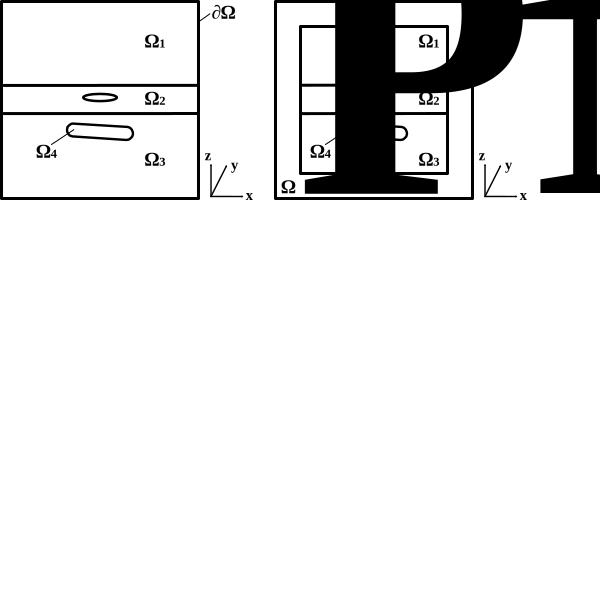
\includegraphics[trim=0mm 0mm 79.0mm 0mm,clip,scale=1]{theory/area_3layers_PML.eps}\label{fig:theory:area_3layers_PML_a}}
	\subfloat[][]{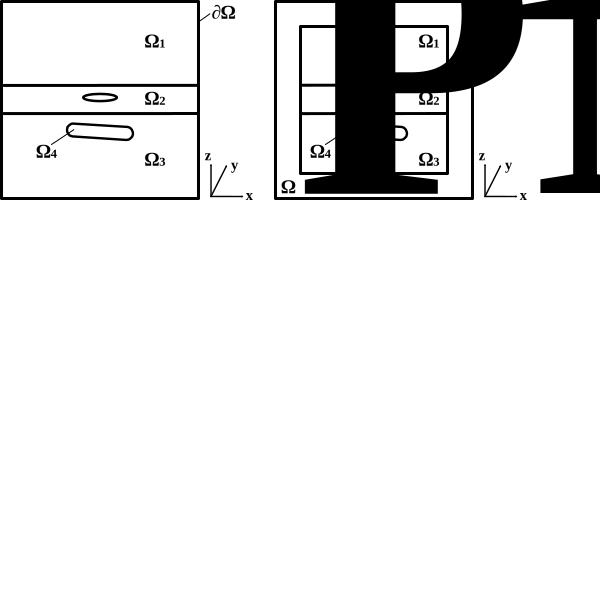
\includegraphics[trim=77.0mm 0mm 0mm 0mm,clip,scale=1]{theory/area_3layers_PML.eps}\label{fig:theory:area_3layers_PML_b}}
	\caption{расчетные области: (а) без PML-слоя и (б) с PML-слоем}
	\label{fig:theory:area_3layers_PML}
\end{figure}

PML-слой определяется модифицированными координатами $\tilde{x}$, $\tilde{y}$, $\tilde{z}$, полученными следующей заменой координат ~\citep{wiik_dehoop_ursin}:
\begin{equation*}
	\tilde{x} = \int\limits_0^x s_x (t) \,dt ,
	\text{~~~~~}
	\tilde{y} = \int\limits_0^y s_y (t) \,dt ,
	\text{~~~~~}
	\tilde{z} = \int\limits_0^z s_z (t) \,dt ,
\end{equation*}
где $s_j(\tau) = 1$ вне PML-слоя, а внутри него может быть задано в виде:
\begin{equation}
	s_j(\tau) = 1 + \chi \left( \frac{d(\tau)}{\delta} \right)^m , \text{~~} m \geq 1 ,
	\label{eq:pml_s}
\end{equation}
где $d(\tau)$ -- расстояние в $j$-м направлении от внутренней границы PML-слоя, $\delta$ -- толщина PML-слоя, $\chi$ -- некоторое комплексное число, причем $\Re(\chi) \ge 0$, $\Im(\chi) \ge 0$. Оператор $\nabla$ в новых координатах будет иметь вид:
\begin{equation*}
	\tilde{\nabla} = \left[ \frac{1}{s_x} \frac{\partial}{\partial x} \,, \frac{1}{s_y} \frac{\partial}{\partial y} \,, \frac{1}{s_z} \frac{\partial}{\partial z} \right] .
\end{equation*}
После такой замены, внутри PML-слоя уравнение Гельмгольца (\ref{eq:helmholtz}) будет иметь вид (\ref{eq:helmholtz_pml})
\begin{equation}
	\tilde{\nabla} \times ( \mu^{-1} \tilde{\nabla} \times \tilde{\mathbf{E}} ) + k^{2} \tilde{\mathbf{E}} = 0 , \label{eq:helmholtz_pml}
\end{equation}
что приведет к преобразованию уравнения (\ref{eq:weak}) к виду (\ref{eq:weak_pml}):
\begin{equation}
	\int\limits_{{\Omega^{PML}}} \mu^{-1} \tilde{\nabla} \times \tilde{\mathbf{E}} \cdot \tilde{\nabla} \times \overline{\mathbf{v}} \,d{\Omega^{PML}} + \int\limits_{{\Omega^{PML}}} k^{2} \tilde{\mathbf{E}} \cdot \overline{\mathbf{v}} \,d{\Omega^{PML}} = 0 . \label{eq:weak_pml}
\end{equation}

В результате, если обозначить $\widehat{\Omega} = \Omega \setminus {\Omega^{PML}}$, то векторная вариационная постановка с учетом PML-слоя примет вид: \textbf{\textit{Найти $\mathbf{E} \in \mathbb{H}_{0}( \mathrm{rot}\,, \widehat{\Omega} )$ и  $\tilde{\mathbf{E}} \in \mathbb{H}_{0}( \mathrm{rot}\,, {\Omega^{PML}} )$, такие что $\forall \mathbf{v} \in \mathbb{H}_{0}( \mathrm{rot}\,, \widehat{\Omega} )$ и $\forall \tilde{\mathbf{v}} \in \mathbb{H}_{0}( \mathrm{rot}\,, {\Omega^{PML}} )$ будет выполнено}}:
\begin{equation*}
	\begin{cases}
		\displaystyle
		\int\limits_{\widehat{\Omega}} \mu^{-1} \nabla \times \mathbf{E} \cdot \nabla \times \overline{\mathbf{v}} \,d\widehat{\Omega} + \int\limits_{\widehat{\Omega}} k^{2} \mathbf{E} \cdot \overline{\mathbf{v}} \,d\widehat{\Omega} = - \int\limits_{\widehat{\Omega}} i \omega \mathbf{J} \cdot \overline{\mathbf{v}} \,d\widehat{\Omega} \\
		\displaystyle
		\int\limits_{{\Omega^{PML}}} \mu^{-1} \tilde{\nabla} \times \tilde{\mathbf{E}} \cdot \tilde{\nabla} \times \tilde{\overline{\mathbf{v}}} \,d{\Omega^{PML}} + \int\limits_{{\Omega^{PML}}} k^{2} \tilde{\mathbf{E}} \cdot \tilde{\overline{\mathbf{v}}} \,d{\Omega^{PML}} = 0 . \\
	\end{cases}
\end{equation*}

% =============================================================================

\subsection{Дискретная вариационная постановка}
Разобьем область $\Omega$ на $m$ непересекающихся элементов:
\begin{equation*}
	\Omega = \bigcup\limits_{k=1}^{m} \Omega_k , \text{~~} \forall i \neq j , \text{~~} \Omega_i \cap \Omega_j = \varnothing .
\end{equation*}

Введем конечномерные подпространства:
\begin{equation*}
	\mathbb{H}_{0}^h( \mathrm{rot}\,, \Omega ) \subset \mathbb{H}_{0}( \mathrm{rot}\,, \Omega ) , \text{~~}
	\mathbb{H}_{0}^h( \mathrm{grad}\,, \Omega ) \subset \mathbb{H}_{0}( \mathrm{grad}\,, \Omega ) .
\end{equation*}
Для дискретных подпространств $\mathbb{H}_{0}^h( \mathrm{rot}\,, \Omega )$ и $\mathbb{H}_{0}^h( \mathrm{grad}\,, \Omega )$ комплекс Де Рама~(\ref{eq:derham}) также будет верен, следовательно закон сохранения заряда~(\ref{eq:charge}) будет также выполнен в слабом смысле~\citep{epov}.

Пространство $\mathbb{H}_{0}^h( \mathrm{rot}\,, \Omega )$ является прямой суммой подпространств~\citep{hiptmair,epov}
\begin{equation}
	\mathbb{H}_{0}^h( \mathrm{rot}\,, \Omega ) = \mathbb{N}_{0}^h( \mathrm{rot}\,, \Omega ) \oplus (\mathbb{N}_{0}^h( \mathrm{rot}\,, \Omega ))^{\bot} ,
	\label{eq:subspaces_sum}
\end{equation}
где $\mathbb{N}_{0}^h( \mathrm{rot}\,, \Omega )$ -- ядро rot-оператора, $(\mathbb{N}_{0}^h( \mathrm{rot}\,, \Omega ))^{\bot}$ -- его ортогональное дополнение. Для выполнения условий непрерывности (\ref{eq:maxwell:tangent_E})-(\ref{eq:maxwell:normal_D}) необходимо использовать полный базис (базис II типа) \citep{webb1993,webb1999,nedelec1980,nedelec1986,epov}, состоящий из двух типов базисных функций. Первый тип -- роторные базисные функции из пространства $(\mathbb{N}_{0}^h( \mathrm{rot}\,, \Omega ))^{\bot}$, которые обеспечивают непрерывность тангенциальных компонент электрического поля $\mathbf{E}$ (\ref{eq:maxwell:tangent_E}). Второй -- градиентные базисные функции из пространства $\mathbb{N}_{0}^h( \mathrm{rot}\,, \Omega )$, которые обеспечивают скачок нормальной компоненты электрического поля $\mathbf{E}$~(\ref{eq:maxwell:normal_D}) и выполнение закона сохранения заряда~(\ref{eq:charge}).

Представим векторнозначную функцию $\mathbf{E}^h$ в виде разложения по базису \linebreak $\boldsymbol{\psi}_j \in \mathbb{H}_{0}^h( \mathrm{rot}\,, \Omega )$:
\begin{equation*}
	\mathbf{E}^h = \sum\limits_{j = 1}^n q_j \boldsymbol{\psi}_j .
\end{equation*}
В качестве тестовой функции выберем базисную функцию $\boldsymbol{\psi}_i \in \mathbb{H}_{0}^h( \mathrm{rot}\,, \Omega )$, тогда конечноэлементная аппроксимация вариационного уравнения (\ref{eq:weak}) примет вид:
\begin{equation}
	\begin{array}{c} { \displaystyle
		\sum\limits_{j = 1}^n \left( \int\limits_\Omega \mu^{-1} \nabla \times \boldsymbol{\psi}_j \cdot \nabla \times \boldsymbol{\psi}_i \,d\Omega + \int\limits_\Omega k^{2} \boldsymbol{\psi}_j \cdot \boldsymbol{\psi}_i \,d\Omega \right) q_j =
	} \\ { \displaystyle
		=  - \int\limits_\Omega i \omega \mathbf{J} \cdot \boldsymbol{\psi}_i \,d\Omega .
	} \end{array}
	\label{eq:weak_discr}
\end{equation}

В матрично-векторной форме (\ref{eq:weak_discr}) можно представить в виде следующей системы линейных алгебраических уравнений (СЛАУ):
\begin{equation}
	( \mathbf{G} + \mathbf{M} )\mathbf{q} = \mathbf{f} , \label{eq:form_29}
\end{equation}
%где:
\begin{equation*}
	\mathbf{G}_{ i,j } = \int\limits_{\Omega_k} \mu^{-1} \nabla \times \mathbf{w}_i \cdot \nabla \times \mathbf{w}_j \,d\Omega_k , \text{~~~}
	\mathbf{M}_{ i,j } = \int\limits_{\Omega_k} k^2 \mathbf{w}_i \cdot \mathbf{w}_j \,d\Omega_k . \label{eq:local_matrixes}
\end{equation*}

Матрица СЛАУ будет иметь симметричную разреженную структуру, поэтому ее удобно хранить в формате CSLR~(Compressed Sparse (Lower triangle) Row) или CSR~(Compressed Sparse Row)~\citep{balandin_slae}.
% Система линейных алгебраических уравнений (СЛАУ) (\ref{eq:slae}) решается специальным двухуровневым методом~\citep{nechaev}.

% =============================================================================

\subsection{Тетраэдральные конечные элементы}

В качестве конечных элементов для представления расчетной области, будем пользоваться тетраэдрами. На тетраэдральном конечном элементе определим $\mathcal{L}$-ко\-ор\-ди\-на\-ты, называемые также барицентрическими координатами~\citep{soloveychick}. Введем нумерацию вершин и ребер, показанную на рисунке \ref{fig:theory:tetrahedron}:
\begin{figure}[H]
	\centering
	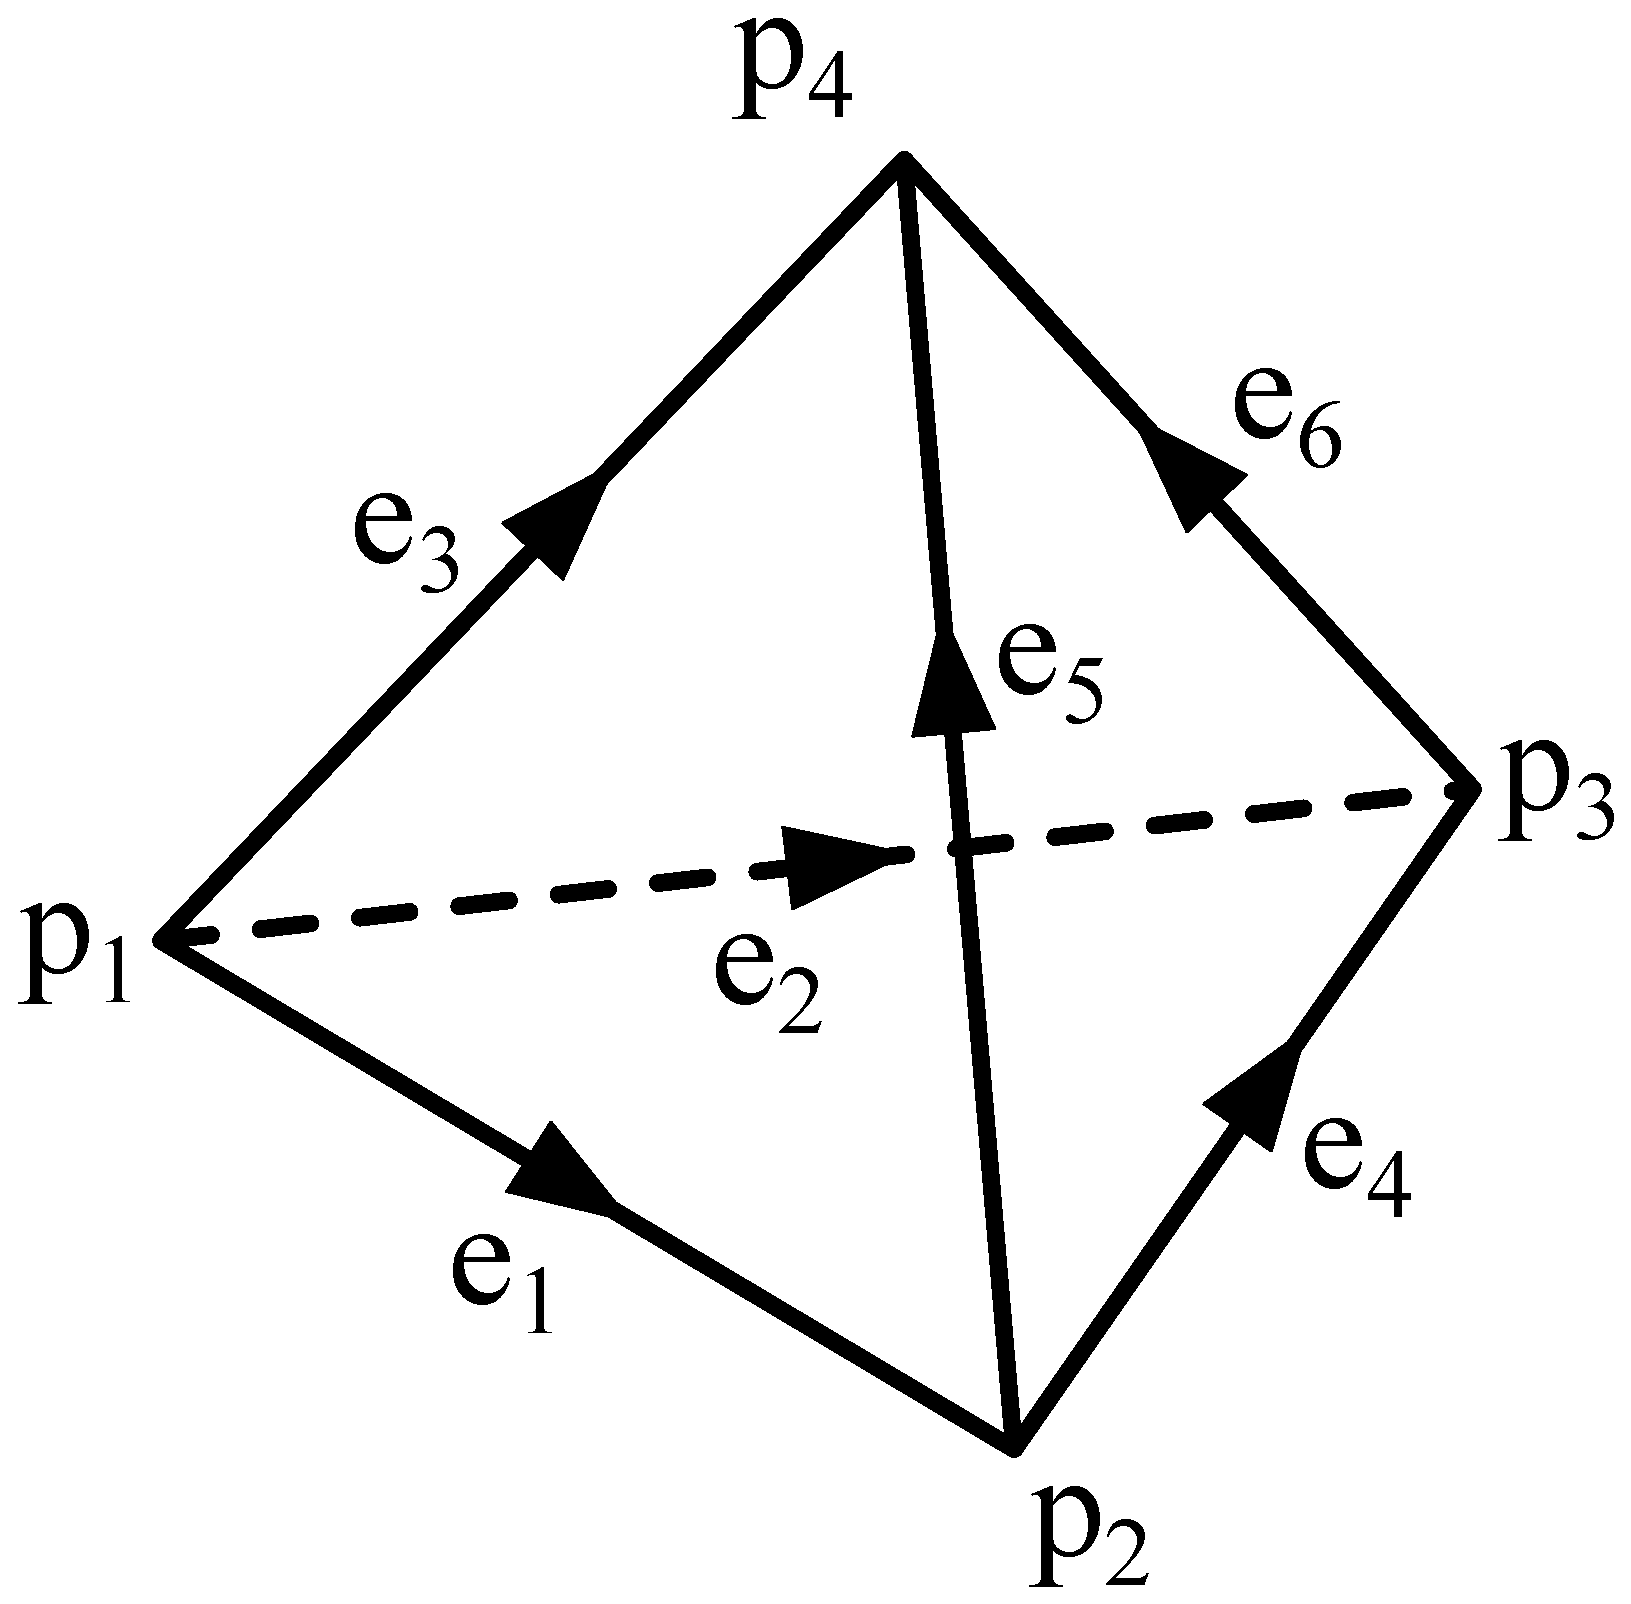
\includegraphics[scale=0.25]{theory/tetrahedron.eps}
	\caption{тетраэдральный конечный элемент}
	\label{fig:theory:tetrahedron}
\end{figure}

\noindent Под $\mathcal{L}$-координатами понимают функции следующего вида:
\begin{equation*}
	\mathcal{L}_i (x, y, z) = \alpha_{i, 1} x + \alpha_{i, 2} y + \alpha_{i, 3} z + \alpha_{i, 4} , \text{~~~} i = \overline{1..4} . \label{eq:tet:L}
\end{equation*}
Коэффициенты $\alpha_{i, j}$ могут быть определены по формуле (\ref{eq:tet:D1}):
\begin{equation}
	\left[
	\begin{matrix}
		\alpha_{1, 1} & \alpha_{1, 2} & \alpha_{1, 3} & \alpha_{1, 4} \\
		\alpha_{2, 1} & \alpha_{2, 2} & \alpha_{2, 3} & \alpha_{2, 4} \\
		\alpha_{3, 1} & \alpha_{3, 2} & \alpha_{3, 3} & \alpha_{3, 4} \\
		\alpha_{4, 1} & \alpha_{4, 2} & \alpha_{4, 3} & \alpha_{4, 4} \\
	\end{matrix}
	\right] = \left[
	\begin{matrix}
		{p_1}_x & {p_2}_x & {p_3}_x & {p_4}_x \\
		{p_1}_y & {p_2}_y & {p_3}_y & {p_4}_y \\
		{p_1}_z & {p_2}_z & {p_3}_z & {p_4}_z \\
		1 & 1 & 1 & 1 \\
	\end{matrix}
	\right]^{-1} . \label{eq:tet:D1}
\end{equation}

Задав $\mathcal{L}$-координаты, можно определить на тетраэдре базисные функции. В отличие от узлового метода конечных элементов, в векторном методе конечных элементов базисные функции ассоциированы не с узлами, а с ребрами (edge), гранями (face) и объемами (volume)~\citep{nechaev, webb1999}. Так как будут использованы полные (II типа) базисы первого и второго порядков, то ограничимся рассмотрением только базисных функций, ассоциированных с ребрами и гранями.

Иерархический векторный базис Вебба второго порядка второго типа на тетраэдрах имеет вид~\citep{mikhajlova}:
\begin{equation}
	\begin{matrix}
		\displaystyle
		\mathbf{w}_{i}^{1,\mathrm{I}} = \mathcal{L}_k \nabla \mathcal{L}_l - \mathcal{L}_l \nabla \mathcal{L}_k ;
		\scriptstyle
		\text{~~} i = 1, ..., 6 ; \text{~~} k, l = 1, ..., 4 ; \text{~~} k < l ,\\
		\displaystyle
		\mathbf{w}_{i}^{1,\mathrm{II}} = \mathcal{L}_k \nabla \mathcal{L}_l + \mathcal{L}_l \nabla \mathcal{L}_k ;
		\scriptstyle
		\text{~~} i = 7, ..., 12 ; \text{~~} k, l = 1, ..., 4 ; \text{~~} k < l ,\\
		\displaystyle
		\mathbf{w}_{i}^{2,\mathrm{I}} = \mathcal{L}_k \mathcal{L}_l \nabla \mathcal{L}_j + \mathcal{L}_j \mathcal{L}_l \nabla \mathcal{L}_k - 2 \mathcal{L}_j \mathcal{L}_k \nabla \mathcal{L}_l ;
		\scriptstyle
		\text{~~} i = 13, ..., 16 ; \text{~~} j, k, l = 1, ..., 4 ; \text{~~} j < k < l ,\\
		\displaystyle
		\mathbf{w}_{i}^{2,\mathrm{I}} = \mathcal{L}_k \mathcal{L}_l \nabla \mathcal{L}_j - 2 \mathcal{L}_j \mathcal{L}_l \nabla \mathcal{L}_k + \mathcal{L}_j \mathcal{L}_k \nabla \mathcal{L}_l ;
		\scriptstyle
		\text{~~} i = 17, ..., 20 ; \text{~~} j, k, l = 1, ..., 4 ; \text{~~} j < k < l ,\\
		\displaystyle
		\mathbf{w}_{i}^{2,\mathrm{II}} = \nabla ( \mathcal{L}_j \mathcal{L}_k \mathcal{L}_l ) ;
		\scriptstyle
		\text{~~} i = 21, ..., 24 ; \text{~~} j, k, l = 1, ..., 4 ; \text{~~} j < k < l ,\\
		\displaystyle
		\mathbf{w}_{i}^{2,\mathrm{II}} = \nabla ( \mathcal{L}_j \mathcal{L}_k ( \mathcal{L}_j - \mathcal{L}_k ) ) ;
		\scriptstyle
		\text{~~} i = 25, ..., 30 ; \text{~~} j, k = 1, ..., 4 ; \text{~~} j < k ,
	\end{matrix}
	\label{eq:basis}
\end{equation}
где $\mathbf{w}_{1}^{1,\mathrm{I}}, ..., \mathbf{w}_{6}^{1,\mathrm{I}}$ -- базисные функции первого порядка первого типа, ассоциированные с ребрами, $\mathbf{w}_{7}^{1,\mathrm{II}}, ..., \mathbf{w}_{12}^{1,\mathrm{II}}$ -- базисные функции первого порядка второго типа, ассоциированные с ребрами, $\mathbf{w}_{13}^{2,\mathrm{I}}, ..., \mathbf{w}_{20}^{2,\mathrm{I}}$ -- базисные функции второго порядка первого типа, ассоциированные с гранями, $\mathbf{w}_{21}^{2,\mathrm{II}}, ..., \mathbf{w}_{24}^{2,\mathrm{II}}$ -- базисные функции второго порядка второго типа, ассоциированные с гранями, $\mathbf{w}_{25}^{2,\mathrm{II}}, ..., \mathbf{w}_{30}^{2,\mathrm{II}}$ -- базисные функции второго порядка второго типа, ассоциированные с ребрами. Так как этот базис иерархический, то для получения базиса меньшего порядка следует ограничиться меньшим количеством функций. Так, для базиса первого порядка второго  типа следует использовать функции $\mathbf{w}_{1}^{1,\mathrm{I}}, ..., \mathbf{w}_{12}^{1,\mathrm{II}}$.

Для вычисления интегралов в (\ref{eq:weak_discr}) воспользуемся кубатурной формулой численного интегрирования (формулой Гаусса)~\citep{misovskih}:
\begin{equation*}
	\int\limits_{\Omega_k} f(x, y, z) \,d\Omega_k = \sum\limits_{i = 1}^m f( x_i , y_i , z_i ) w_i ,
\end{equation*}
где $(x_i , y_i , z_i )$ -- точки Гаусса, $m$ -- число точек Гаусса, $w_i$ -- соответствующие веса. При работе с базисными функциями второго порядка нужно использовать формулы, которые бы обеспечивали восьмой порядок интегрирования~\citep{zhang_integration}. Для базисных функций первого порядка будет достаточно и меньших порядков интегрирования~\citep{misovskih}.

% =============================================================================

\subsection{Треугольные конечные элементы}

Границы области $\Omega$ являются двумерными и представляют собой треугольники. Для учета краевых условий (\ref{eq:bound1}) требуется построить разложение $\mathbf{E}^g$ по базису соответствующей границы в смысле МНК, для этого нужно решать СЛАУ вида
\begin{equation}
	\mathbf{M}^{S_1} \tilde{\mathbf{q}} = \mathbf{b}^{S_1} ,
	\label{eq:bound_mnk}
\end{equation}
где $\displaystyle \mathbf{M}^{S_1}_{i,j} = \int\limits_{S_1} \tilde{\mathbf{w}}_i \cdot \tilde{\mathbf{w}}_j \,d S_1$, $\displaystyle \mathbf{b}^{S_1}_{i} = \int\limits_{S_1} \mathbf{E}^g \cdot \tilde{\mathbf{w}}_i \,d S_1$, $\tilde{\mathbf{w}}_i$ и $\tilde{\mathbf{w}}_j$ -- базисные функции на треугольниках.

Определим $\mathcal{L}$-координаты на треугольниках таким же образом, как и на тетраэдрах. Введем нумерацию вершин и ребер согласно рисунку \ref{fig:theory:triangle}:
\begin{figure}[H]
	\centering
	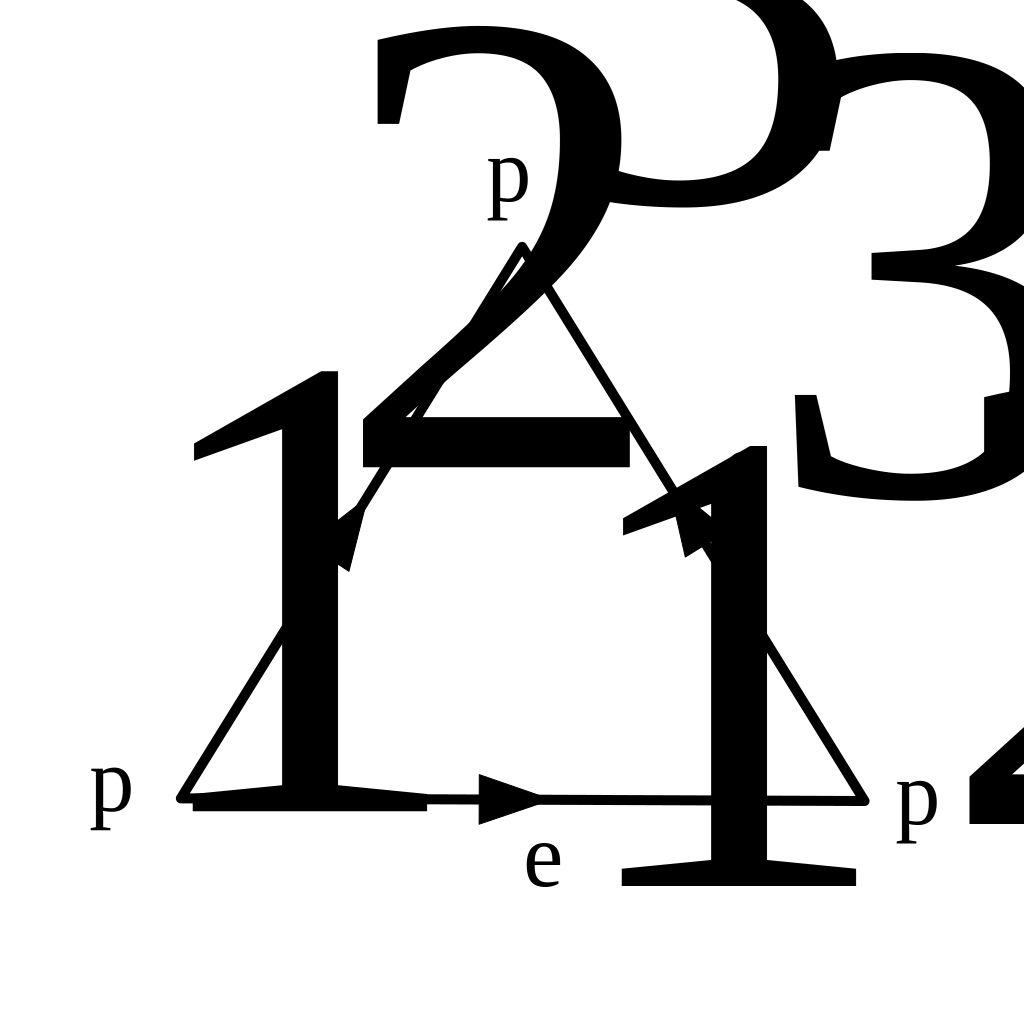
\includegraphics[scale=0.25]{theory/triangle.eps}
	\caption{треугольный конечный элемент}
	\label{fig:theory:triangle}
\end{figure}

\noindent Тогда $\mathcal{L}$-координаты примут вид:
\begin{equation*}
	\mathcal{L}_i (x, y) = \alpha_{i, 1} x + \alpha_{i, 2} y + \alpha_{i, 3} , \text{~~~} i = \overline{1..3} . \label{eq:tr:L}
\end{equation*}
Коэффициенты $\alpha_{i, j}$ могут быть определены по формуле (\ref{eq:tr:D1}):
\begin{equation}
	\left[
	\begin{matrix}
		\alpha_{1, 1} & \alpha_{1, 2} & \alpha_{1, 3} \\
		\alpha_{2, 1} & \alpha_{2, 2} & \alpha_{2, 3} \\
		\alpha_{3, 1} & \alpha_{3, 2} & \alpha_{3, 3} \\
	\end{matrix}
	\right] = \left[
	\begin{matrix}
		{p_1}_x & {p_2}_x & {p_3}_x \\
		{p_1}_y & {p_2}_y & {p_3}_y \\
		1 & 1 & 1 \\
	\end{matrix}
	\right]^{-1} . \label{eq:tr:D1}
\end{equation}

Иерархический векторный базис Вебба второго порядка второго типа на треугольниках имеет вид:
\begin{equation*}
	\begin{matrix}
		\displaystyle
		\tilde{\mathbf{w}}_{i}^{1,\mathrm{I}} = \mathcal{L}_k \nabla \mathcal{L}_l - \mathcal{L}_l \nabla \mathcal{L}_k ;
		\scriptstyle
		\text{~~} i = 1, ..., 3 ; \text{~~} k, l = 1, ..., 3 ; \text{~~} k < l ,\\
		\displaystyle
		\tilde{\mathbf{w}}_{i}^{1,\mathrm{II}} = \mathcal{L}_k \nabla \mathcal{L}_l + \mathcal{L}_l \nabla \mathcal{L}_k ;
		\scriptstyle
		\text{~~} i = 4, ..., 6 ; \text{~~} k, l = 1, ..., 3 ; \text{~~} k < l ,\\
		\displaystyle
		\tilde{\mathbf{w}}_{7}^{2,\mathrm{I}} = \mathcal{L}_2 \mathcal{L}_3 \nabla \mathcal{L}_1 + \mathcal{L}_1 \mathcal{L}_3 \nabla \mathcal{L}_2 - 2 \mathcal{L}_1 \mathcal{L}_2 \nabla \mathcal{L}_3 ,\\
		\displaystyle
		\tilde{\mathbf{w}}_{8}^{2,\mathrm{I}} = \mathcal{L}_2 \mathcal{L}_3 \nabla \mathcal{L}_1 - 2 \mathcal{L}_1 \mathcal{L}_3 \nabla \mathcal{L}_2 + \mathcal{L}_1 \mathcal{L}_2 \nabla \mathcal{L}_3 ,\\
		\displaystyle
		\tilde{\mathbf{w}}_{9}^{2,\mathrm{II}} = \nabla ( \mathcal{L}_1 \mathcal{L}_2 \mathcal{L}_3 ) ,\\
		\displaystyle
		\tilde{\mathbf{w}}_{i}^{2,\mathrm{II}} = \nabla ( \mathcal{L}_j \mathcal{L}_k ( \mathcal{L}_j - \mathcal{L}_k ) ) ;
		\scriptstyle
		\text{~~} i = 10, ..., 12 ; \text{~~} j, k = 1, ..., 3 ; \text{~~} j < k ,
	\end{matrix}
	\label{eq:tr_basis}
\end{equation*}
где $\tilde{\mathbf{w}}_{1}^{1,\mathrm{I}}, ..., \tilde{\mathbf{w}}_{3}^{1,\mathrm{I}}$ -- базисные функции первого порядка первого типа, $\tilde{\mathbf{w}}_{4}^{1,\mathrm{II}}, ..., \tilde{\mathbf{w}}_{6}^{1,\mathrm{II}}$ -- базисные функции первого порядка второго типа, $\tilde{\mathbf{w}}_{7}^{2,\mathrm{I}}, \tilde{\mathbf{w}}_{8}^{2,\mathrm{I}}$ -- базисные функции второго порядка первого типа, $\tilde{\mathbf{w}}_{9}^{2,\mathrm{II}}, ..., \tilde{\mathbf{w}}_{12}^{2,\mathrm{II}}$ -- базисные функции второго порядка второго типа. Для базиса первого порядка второго типа следует использовать функции $\tilde{\mathbf{w}}_{1}^{1,\mathrm{I}}, ..., \tilde{\mathbf{w}}_{6}^{1,\mathrm{II}}$.

Для вычисления интегралов в (\ref{eq:bound_mnk}) воспользуемся формулой Гаусса~\citep{misovskih}:
\begin{equation*}
	\int\limits_{\Omega_k} f(x, y) \,d\Omega_k = \sum\limits_{i = 1}^m f( x_i , y_i) w_i ,
\end{equation*}
где $(x_i , y_i)$ -- точки Гаусса, $m$ -- число точек Гаусса, $w_i$ -- соответствующие веса. Так же, как и для тетраэдров, для работы с базисом второго порядка нужно использовать формулы, обеспечивающие восьмой порядок интегрирования~\citep{zhang_integration}. Для базиса первого порядка достаточно и меньших порядков интегрирования~\citep{misovskih}.

% =============================================================================

\clearpage
\section{Вычислительные эксперименты}
\labelname{3}\label{sec:numerical_experiments}
\subsection{Верификация программного комплекса}
Верификация полученной конечноэлементной аппроксимации будет проводиться на тестовой задаче, имеющей аналитическое решение.
\subsubsection{Расчетная область}
Расчетная область представляет собой куб со следующими параметрами: $x \in [0,1]$, $y \in [0,1]$, $z \in [0,1]$. Куб разбивается на регулярную тетраэдральную сетку согласно рисунку \ref{fig:verify:x1}:

\begin{figure}[!htbp]
%\begin{figure}[H]
	\centering
	% trim=left bottom right top
	\includegraphics[trim=387mm 20mm 5mm 220mm,clip,scale=0.4]{verify/x1.png}
	\caption{конечноэлементная сетка для верификации}
	\label{fig:verify:x1}
\end{figure}

\noindent Всего в сетке 750 тетраэдров, 300 треугольников по границе, 216 узлов, 1115 ребер и 1650 граней.

Физические параметры среды заданы следующим образом: $\varepsilon = \varepsilon_0$, $\mu = \mu_0$, $\sigma = 10$~См/м. Частота источника поля $\nu = \frac{100}{2 \pi}$~Гц. На всех внешних гранях расчетной области заданы краевые условия первого рода (\ref{eq:bound1}).

% =============================================================================

\subsubsection{Тестирование на линейных по пространству функциях}
В качестве аналитического решения уравнения (\ref{eq:helmholtz}) выберем функцию
\begin{equation*}
	\mathbf{E} = ( y+z , x+z, x+y )^T .
\end{equation*}
Тестирование будем проводить на базисных функциях первого и второго порядка второго типа. Погрешности в норме пространства $\mathbb{L}^2$ полученных решений приведены в таблице~\ref{tab:verify:linear_diff}.

\begin{table}[H]
	\caption{относительные погрешности в норме $\mathbb{L}^2$}
	\label{tab:verify:linear_diff}
	\begin{tabularx}{\textwidth}{|C{1}|C{1}|C{1}|C{1}|C{1}|C{1}|}
		\hline Порядок базисных ф-й & \raisebox{-0.7em}{$\smash{\displaystyle \frac{\| \mathbf{E} - \mathbf{E}^h \|_{\mathbb{L}^2}}{\| \mathbf{E} \|_{\mathbb{L}^2}}}$} & \raisebox{-0.7em}{$\smash{\displaystyle \frac{\| \mathbf{E}_x - \mathbf{E}^h_x \|_{\mathbb{L}^2}}{\| \mathbf{E}_x \|_{\mathbb{L}^2}}}$} & \raisebox{-0.7em}{$\smash{\displaystyle \frac{\| \mathbf{E}_y - \mathbf{E}^h_y \|_{\mathbb{L}^2}}{\| \mathbf{E}_y \|_{\mathbb{L}^2}}}$} & \raisebox{-0.7em}{$\smash{\displaystyle \frac{\| \mathbf{E}_z - \mathbf{E}^h_z \|_{\mathbb{L}^2}}{\| \mathbf{E}_z \|_{\mathbb{L}^2}}}$} \\
		\hline 1 & 5.277e-11 & 5.313e-11 & 5.345e-11 & 5.169e-11 \\
		\hline 2 & 8.064e-11 & 8.111e-11 & 8.056e-11 & 8.025e-11 \\
		\hline
	\end{tabularx}
\end{table}
\vspace{-0.5cm}Как и следовало ожидать, метод хорошо аппроксимировал линейную по пространству функцию.

% =============================================================================

\subsubsection{Тестирование на полиномиальных функциях}

В качестве аналитического решения уравнения (\ref{eq:helmholtz}) выберем функцию
\begin{equation}
	\mathbf{E} = \left( \begin{array}{c}
		e^{-(0.5-y)^2 -(0.5-z)^2} \\
		e^{-(0.5-x)^2 -(0.5-z)^2} \\
		e^{-(0.5-x)^2 -(0.5-y)^2} \\
	\end{array} \right) .
	\label{eq:verify:exp_solution}
\end{equation}
Тестирование будем проводить на базисных функциях первого и второго порядка второго типа. Погрешности в норме пространства $\mathbb{L}^2$ полученных решений приведены в таблице~\ref{tab:verify:exp_diff}.

\begin{table}[H]
	\caption{относительные погрешности в норме $\mathbb{L}^2$}
	\label{tab:verify:exp_diff}
	\begin{tabularx}{\textwidth}{|C{1}|C{1}|C{1}|C{1}|C{1}|C{1}|}
		\hline Порядок базисных ф-й & \raisebox{-0.7em}{$\smash{\displaystyle \frac{\| |\mathbf{E}| - |\mathbf{E}^h| \| {\mathbb{L}^2}}{\| |\mathbf{E}| \|_{\mathbb{L}^2}}}$} & \raisebox{-0.7em}{$\smash{\displaystyle \frac{\| \mathbf{E}_x - \mathbf{E}^h_x \|_{\mathbb{L}^2}}{\| \mathbf{E}_x \|_{\mathbb{L}^2}}}$} & \raisebox{-0.7em}{$\smash{\displaystyle \frac{\| \mathbf{E}_y - \mathbf{E}^h_y \|_{\mathbb{L}^2}}{\| \mathbf{E}_y \|_{\mathbb{L}^2}}}$} & \raisebox{-0.7em}{$\smash{\displaystyle \frac{\| \mathbf{E}_z - \mathbf{E}^h_z \|_{\mathbb{L}^2}}{\| \mathbf{E}_z \|_{\mathbb{L}^2}}}$} \\
		\hline 1 & 6.608e-3 & 7.869e-3 & 5.877e-3 & 5.877e-3 \\
		\hline 2 & 1.775e-4 & 1.895e-4 & 1.712e-4 & 1.712e-4 \\
		\hline
	\end{tabularx}
\end{table}
\vspace{-0.5cm}Метод достаточно хорошо аппроксимировал и не полиномиальных функцию.

% =============================================================================

\subsubsection{Определение порядка аппроксимации}

В качестве аналитического решения уравнения (\ref{eq:helmholtz}) выберем функцию (\ref{eq:verify:exp_solution}). Проведем исследование на порядок аппроксимации. Измельчим сетку расчетной области, изображенную на рисунке \ref{fig:verify:x1}, в 2 и 4 раза, после чего сравним погрешности полученных решений. Измельченные сетки приведены на рисунках \ref{fig:verify:x2} и \ref{fig:verify:x4}, погрешности в норме пространства $\mathbb{L}^2$ полученных решений и порядок аппроксимации -- в таблице \ref{tab:verify:exp_order}.

\begin{table}[H]
	\caption{относительные погрешности в норме $\mathbb{L}^2$}
	\label{tab:verify:exp_order}
	\begin{tabularx}{\textwidth}{|C{0.7}|C{0.9}|C{0.9}|C{0.9}|C{1.3}|C{1.3}|}
		\hline Порядок базиса &
		\raisebox{-0.7em}{$\smash{\frac{\| \mathbf{E} - \mathbf{E}^{h} \|{\mathbb{L}^2}}{\| \mathbf{E} \|_{\mathbb{L}^2}}}$} &
		\raisebox{-0.7em}{$\smash{\frac{\| \mathbf{E} - \mathbf{E}^{h/2} \|_{\mathbb{L}^2}}{\| \mathbf{E} \|_{\mathbb{L}^2}}}$} &
		\raisebox{-0.7em}{$\smash{\frac{\| \mathbf{E} - \mathbf{E}^{h/4} \|_{\mathbb{L}^2}}{\| \mathbf{E} \|_{\mathbb{L}^2}}}$} &
		\raisebox{-0.7em}{$\smash{\log_2 \frac{\| \mathbf{E} - \mathbf{E}^{h} \|_{\mathbb{L}^2}}{\| \mathbf{E} - \mathbf{E}^{h/2} \|_{\mathbb{L}^2}}}$} &
		\raisebox{-0.7em}{$\smash{\log_2 \frac{\| \mathbf{E} - \mathbf{E}^{h/2} \|_{\mathbb{L}^2}}{\| \mathbf{E} - \mathbf{E}^{h/4} \|_{\mathbb{L}^2}}}$} \\
		\hline 1 & 6.608e-3 & 1.637e-3 & 5.051e-4 & 2.013 & 1.696 \\
		\hline 2 & 1.775e-4 & 2.164e-5 & 3.582e-6 & 3.036 & 2.595 \\
		\hline
	\end{tabularx}
\end{table}
\vspace{-0.5cm}

\begin{figure}[H]
	\centering
	% trim=left bottom right top
	\subfloat[][]{\includegraphics[trim=387mm 20mm 5mm 220mm,clip,scale=0.4]{verify/x2.png}\label{fig:verify:x2}}
	~~~~~
	\subfloat[][]{\includegraphics[trim=387mm 20mm 5mm 220mm,clip,scale=0.4]{verify/x4.png}\label{fig:verify:x4}}
	\caption{конечноэлементные сетки для определения порядка аппроксимации}
	\label{fig:verify:x2_x4}
\end{figure}

Из результатов видно, что порядок аппроксимации получился второй для базисных функций первого порядка и третий для базисных функций второго порядка, что совпадает с теоретическими значениями.

% =============================================================================

\subsection{Исследование влияния слоя воздуха}

Проведем исследование влияния слоя воздуха в модельной задаче морской геоэлектрики при различной глубине погружения в воду источника электромагнитного возмущения.

В этом исследовании будем пользоваться базисными функциями второго полного порядка.

\subsubsection{Описание расчетной области}
Схематичное изображение расчетной области показано на рисунке \ref{fig:res1:area}, где $\Omega_1$ -- воздух ($\sigma=10^{-6}$ См/м, $\mu=\mu_0$, $\varepsilon=\varepsilon_0$); $\Omega_2$ -- морская вода ($\sigma=3.3$ См/м, $\mu=\mu_0$, $\varepsilon=\varepsilon_0$); $\Omega_3$ -- грунт ($\sigma=0.2$ См/м, $\mu=\mu_0$, $\varepsilon=\varepsilon_0$); $\Omega_4$ -- углеводороды ($\sigma=10^{-2}$~См/м, $\mu=\mu_0$, $\varepsilon=\varepsilon_0$); $L_1$, $L_2$ и $L_3$ -- размеры области моделирования по осям $x$, $y$ и $z$ соответственно; $L_1 = L_2 = L_3 = 6000$~м; $h_1=600$~м -- толщина $\Omega_2$; $l_1=400$~м, $h_3=75$~м, $h_2=135$~м -- длина, толщина и глубина объекта $\Omega_4$ соответственно.

\begin{figure}[H]
	\centering
	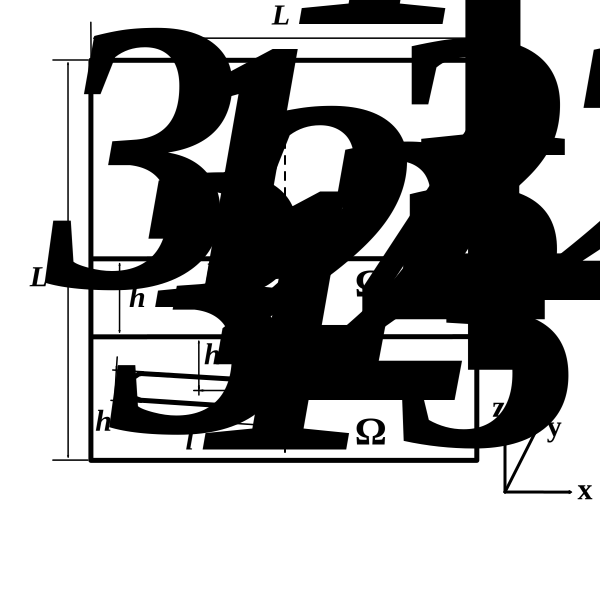
\includegraphics[scale=0.5]{research-1/area_3layers_shift_3.eps}
	\caption{схематичное изображение расчетной области}
	\label{fig:res1:area}
\end{figure}

\noindent Объект $\Omega_4$ представляет собой скругленный прямоугольный параллелепипед с двумя равными сторонами, наклоненный под углом $5^{\circ}$. Источником электрического поля является токовая петля диаметром $d=100$~м с током частотой 1~Гц, глубина $h$ которой варьируется в ходе исследования.

\subsubsection{Конечноэлементная сетка}
Фрагмент $x \in [-600,0]$, $y \in [-600,600]$ $z \in [-1000,600]$ одной из конечноэлементных сеток, использованных для проведения исследования, представлен на рисунке \ref{fig:res1:mesh}.

\begin{figure}[H]
	\centering
	% trim=left bottom right top
	\includegraphics[trim=390mm 20mm 5mm 195mm,clip,scale=0.45]{research-1/mesh/mesh.png}
	\caption{фрагмент конечноэлементной сетки}
	\label{fig:res1:mesh}
\end{figure}

\subsubsection{Результаты исследования}
Разности решений в норме $\mathbb{L}^2$ в объеме $[-600,600] \times [-600,600] \times [-1000,0]$ между областью, в которой присутствует слой воздуха, и областью, в которой заданы условия непротекания~(\ref{eq:bound2}), для некоторых значений глубины петли $h$ показаны в таблице \ref{tab:res1:diff}. В форме графика эти данные приведены на рисунке \ref{fig:res1:graph}.

\begin{figure}[H]
	\centering
	\includegraphics[scale=1]{research-1/presentation/presentation.eps}
	\caption{график изменения относительной разности решений при изменении глубины}
	\label{fig:res1:graph}
\end{figure}

\begin{table}[H]
	\caption{относительные разности решений}
	\label{tab:res1:diff}
	\begin{tabularx}{\textwidth}{|C{2.4}|C{0.8}|C{0.8}|C{0.8}|C{0.8}|C{0.8}|C{0.8}|C{0.8}|}
		\hline Глубина петли & 5 & 10 & 50 & 100 & 200 & 300 & 400 \\
		\hline $\displaystyle \frac{\| | \mathbf{E}^{air} - \mathbf{E}^{noair} | \|_{\mathbb{L}^2}}{\| | \mathbf{E}^{air} | \|_{\mathbb{L}^2}}$ & 0.44 & 0.40 & 0.24 & 0.14 & 0.07 & 0.04 & 0.02 \\
		\hline
	\end{tabularx}
\end{table}

Графики вещественной компоненты $\mathbf{E}_y$ по линии $y=0$, $z=-610$ для различных глубин петли представлены на рисунках \ref{fig:res1:5_50} и \ref{fig:res1:200_300}.

\begin{figure}[H]
	\centering
	\subfloat[][]{\includegraphics[scale=1]{research-1/-5/EyR_-700.eps}\label{fig:res1:5}}
	~
	\subfloat[][]{\includegraphics[scale=1]{research-1/-50/EyR_-700.eps}\label{fig:res1:50}}
	\caption{$\Re(\mathbf{E}_y)$ по линии $y=0$, $z=-610$, глубина (а) 5 м и (б) 50 м}
	\label{fig:res1:5_50}
\end{figure}

\vspace{-0.8cm}

\begin{figure}[H]
	\centering
	\subfloat[][]{\includegraphics[scale=1]{research-1/-200/EyR_-700.eps}\label{fig:res1:200}}
	~
	\subfloat[][]{\includegraphics[scale=1]{research-1/-300/EyR_-700.eps}\label{fig:res1:300}}
	\caption{$\Re(\mathbf{E}_y)$ по линии $y=0$, $z=-610$, глубина (а) 200 м и (б) 300 м}
	\label{fig:res1:200_300}
\end{figure}

Из результатов следует, что слой воздуха оказывает значительное влияние на получаемое решение при расположении источника электромагнитного возмущения на малой глубине (меньше трехсот метров для рассмотренной конфигурации).

% =============================================================================

\subsection{Исследование эффективности применения PML-слоя}
Цель вычислительных экспериментов: определение эффективности применения PML-слоя. Геометрические характеристики PML-слоя показаны на рисунке \ref{fig:res2:info_2d}.
\begin{figure}[H]
	\centering
	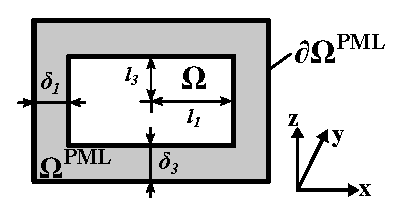
\includegraphics[scale=1]{research-2/info_2d/info_2d_2.eps}
	\caption{геометрические характеристики PML-слоя}
	\label{fig:res2:info_2d}
\end{figure}

Вычислительные эксперименты проводились следующим образом: последовательно варьировался каждый из параметров PML-слоя: толщина слоя в $k$-м направлении $\delta_k$, где $k = \begin{smallmatrix}x\\1\end{smallmatrix},\begin{smallmatrix}y\\2\end{smallmatrix},\begin{smallmatrix}z\\3\end{smallmatrix}$, расстояние от центра области до внутренних границ слоя $l_k$, коэффициент комплексного растяжения координат $\chi$~(\ref{eq:pml_s}), оставшиеся параметры фиксировались, что позволило определить параметры, оказывающие наибольшее влияние на характеристики PML-слоя.

Фрагменты тетраэдральных конечноэлементных сеток с <<большим баком>> и с PML-слоем приведены на рисунках \ref{fig:res2:meshes_a} и \ref{fig:res2:meshes_b}.

\begin{figure}[H]
	\centering
	% trim=left bottom right top
	\subfloat[][]{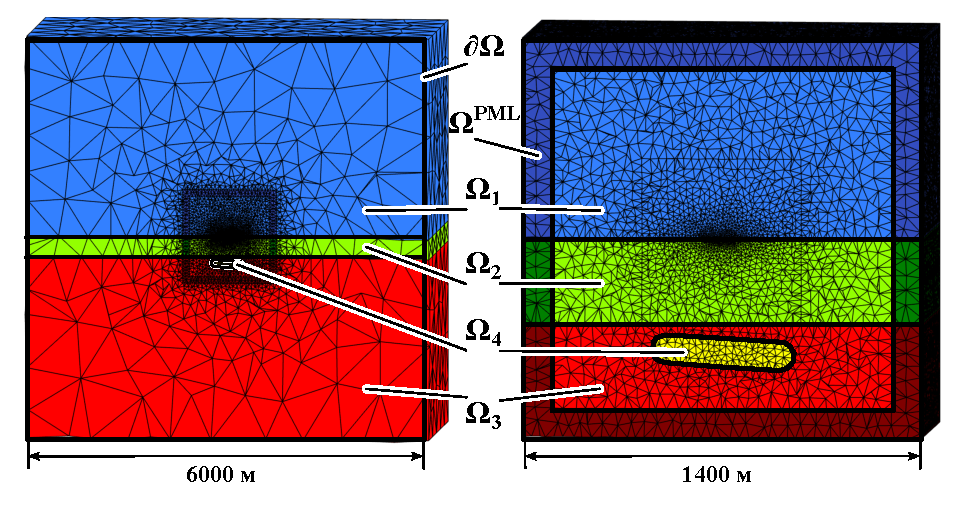
\includegraphics[trim=0mm 0mm 79.2mm 0mm,clip,scale=1]{research-2/meshes/meshes_color.eps}\label{fig:res2:meshes_a}}
	\subfloat[][]{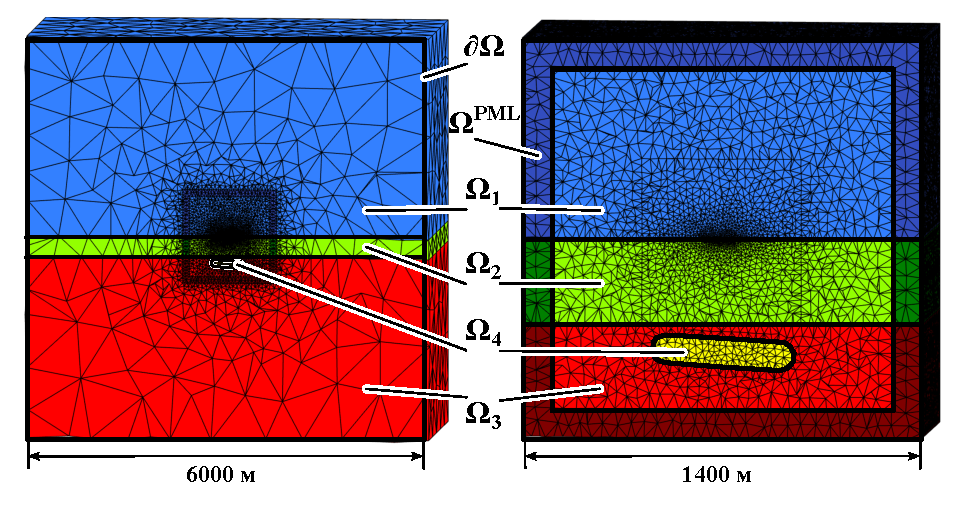
\includegraphics[trim=79.2mm 0mm 0mm 0mm,clip,scale=1]{research-2/meshes/meshes_color.eps}\label{fig:res2:meshes_b}}
	\caption{конечноэлементные сетки: (а) <<большой бак>> и (б) PML-слой}
	\label{fig:res2:meshes}
\end{figure}

В этом исследовании будем пользоваться базисными функциями первого полного порядка.

\subsubsection{Описание расчетной области}
Схематичное изображение расчетной области показано на рисунке \ref{fig:res2:area}, где $\Omega_1$ -- воздух ($\sigma=10^{-6}$ См/м, $\mu=\mu_0$, $\varepsilon=\varepsilon_0$); $\Omega_2$ -- морская вода ($\sigma=3.3$ См/м, $\mu=\mu_0$, $\varepsilon=\varepsilon_0$); $\Omega_3$ -- грунт ($\sigma=0.2$ См/м, $\mu=\mu_0$, $\varepsilon=\varepsilon_0$); $\Omega_4$ -- углеводороды ($\sigma=10^{-2}$~См/м, $\mu=\mu_0$, $\varepsilon=\varepsilon_0$); $L_1$, $L_2$ и $L_3$ -- размеры области моделирования по осям $x$, $y$ и $z$ соответственно; $L_1 = L_2 = L_3 = 6000$~м; $h_1=300$~м -- толщина $\Omega_2$; $l_1=400$~м, $h_3=100$~м, $h_2=100$~м -- длина, толщина и глубина объекта $\Omega_4$ соответственно.

\begin{figure}[H]
	\centering
	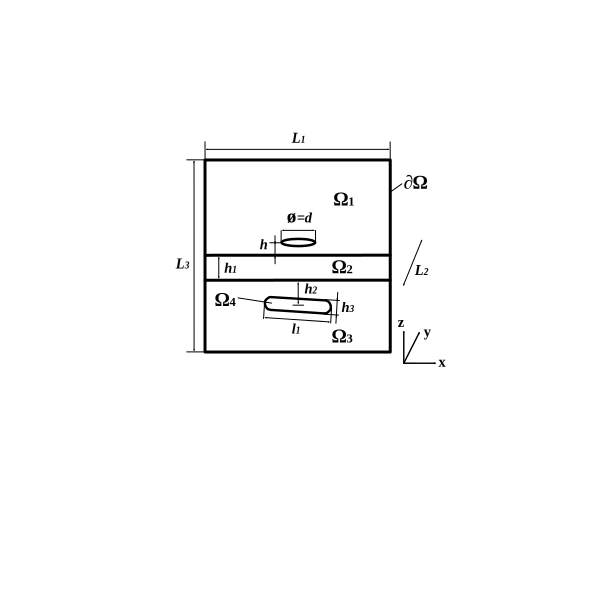
\includegraphics[scale=1]{research-2/area_3layers/area_3layers_3.eps}
	\caption{расчетная область}
	\label{fig:res2:area}
\end{figure}

Объект $\Omega_4$ представляет собой скругленный прямоугольный параллелепипед с двумя равными сторонами, наклоненный под углом $5^{\circ}$. Источником электрического поля является петля диаметром $d = 100$~м с током частотой $1$~Гц, расположенная в воздухе на расстоянии $h = 5$~м от границы раздела сред воздух-вода. Также рассматривается случай, когда петля расположена в воде ($h = -5$~м).

Выделим внутри области c условием <<большого бака>> и области, на границе которой задан PML-слой, подобласть $\Omega'$ размером $1000 \times 1000 \times 1000$~м${}^3$. Для этой подобласти в данном исследовании будем оценивать разность в норме $\mathbb{L}^2$ между действительными компонентами $\mathbf{E}_y$ векторов решений $\mathbf{E}_y^{\text{бак}}$ и $\mathbf{E}_y^{\text{PML}}$, полученных с применением <<большого бака>> и PML-слоя соответственно.

\subsubsection{Варьирование коэффициентов растяжения}
Зафиксируем $\delta_k = 100$~м, $l_k = 600$~м, $m = 3$, $h = 5$~м и будем варьировать коэффициент комплексного растяжения координат $\chi$. Размер получаемой СЛАУ для <<большого бака>> -- 653814, с PML-слоем -- 616180. Результаты приведены в таблице \ref{tab:res2:chi_5}. Для случая $h= -5$~м размер получаемой СЛАУ для <<большого бака>> -- 652396, с PML-слоем -- 614504. Результаты приведены в таблице \ref{tab:res2:chi_m5}.
\begin{table}[H]
	\caption{варьирование коэффициентов растяжения при $h= 5$~м}
	\label{tab:res2:chi_5}
	\begin{spacing}{1.2}
	\setlength{\parskip}{0pt}
	\fontsize{12}{14}\selectfont
	\begin{tabularx}{\textwidth}{|C{0.65}|C{0.65}|C{0.65}|C{0.65}|C{0.65}|C{0.65}|C{3.1}|C{1}|C{1}|}
		\rowcolor[gray]{.9} \hline $\Re(\chi)$ в $\Omega_1$ & $\Im(\chi)$ в $\Omega_1$ & $\Re(\chi)$ в $\Omega_2$ & $\Im(\chi)$ в $\Omega_2$ & $\Re(\chi)$ в $\Omega_3$ & $\Im(\chi)$ в $\Omega_3$ & \raisebox{-0.8em}{$\smash{\displaystyle \frac{\lVert \Re(\mathbf{E}_y^{\text{бак}}) - \Re(\mathbf{E}_y^{\text{PML}})\rVert}{\lVert \Re(\mathbf{E}_y^{\text{бак}})\rVert}}$} & Время, бак & Время, PML \\[0.2em]
		\hline 3 & 0 & 1 & 5 & 3 & 1 & 0.106636 & \multirow{4}{*}{650} & 592 \\
		\cline{1-7}\cline{9-9} 3 & 1 & 0 & 6 & 2 & 1 & 0.0925 & & 599 \\
		\cline{1-7}\cline{9-9} 4 & 0 & 1 & 5 & 3 & 1 & 0.0947 & & 731 \\
		\cline{1-7}\cline{9-9} 4 & 1 & 0 & 6 & 2 & 1 & 0.0910 & & 591 \\
		\hline
	\end{tabularx}
	\end{spacing}
\end{table}

\begin{table}[H]
	\caption{варьирование коэффициентов растяжения при $h= -5$~м}
	\label{tab:res2:chi_m5}
	\begin{spacing}{1.2}
	\setlength{\parskip}{0pt}
	\fontsize{12}{14}\selectfont
	\begin{tabularx}{\textwidth}{|C{0.65}|C{0.65}|C{0.65}|C{0.65}|C{0.65}|C{0.65}|C{3.1}|C{1}|C{1}|}
		\rowcolor[gray]{.9} \hline $\Re(\chi)$ в $\Omega_1$ & $\Im(\chi)$ в $\Omega_1$ & $\Re(\chi)$ в $\Omega_2$ & $\Im(\chi)$ в $\Omega_2$ & $\Re(\chi)$ в $\Omega_3$ & $\Im(\chi)$ в $\Omega_3$ & \raisebox{-0.8em}{$\smash{\displaystyle \frac{\lVert \Re(\mathbf{E}_y^{\text{бак}}) - \Re(\mathbf{E}_y^{\text{PML}})\rVert}{\lVert \Re(\mathbf{E}_y^{\text{бак}})\rVert}}$} & Время, бак & Время, PML \\[0.2em]
		\hline 4 & 0 & 1 & 5 & 3 & 1 & 0.0929047 & \multirow{4}{*}{309} & 344 \\
		\cline{1-7}\cline{9-9} 4 & 0 & 1 & 6 & 3 & 1 & 0.0870 & & 294 \\
		\cline{1-7}\cline{9-9} 4 & 0 & 1 & 6 & 3 & 2 & 0.0809 & & 253 \\
		\cline{1-7}\cline{9-9} 4 & 1 & 1 & 6 & 3 & 2 & 0.0658 & & 306 \\
		\hline
	\end{tabularx}
	\end{spacing}
\end{table}

\subsubsection{Варьирование толщины PML-слоя}
Зафиксируем $\chi_{\Omega_1} = (4, 1)$, $\chi_{\Omega_2} = (0, 6)$, $\chi_{\Omega_3} = (2, 1)$, $l_k = 600$~м, $m = 3$, $h = 5$~м и будем варьировать толщину PML-слоя $\delta_k$. Результаты приведены в таблице \ref{tab:res2:delta_5}. Для случая $h= -5$~м выберем $\chi_{\Omega_1} = (4, 0)$, $\chi_{\Omega_2} = (1, 6)$, $\chi_{\Omega_3} = (3, 2)$. Результаты приведены в таблице \ref{tab:res2:delta_m5}.

\begin{table}[H]
	\caption{варьирование толщины PML-слоя при $h= 5$~м}
	\label{tab:res2:delta_5}
	\begin{spacing}{1.2}
	\setlength{\parskip}{0pt}
	\fontsize{12}{14}\selectfont
	\begin{tabularx}{\textwidth}{|C{0.4}|C{2.0}|C{0.8}|C{0.8}|C{1.0}|C{1.0}|}
		\rowcolor[gray]{.9} \hline \raisebox{-0.8em}[0.8em]{$\smash{\displaystyle \delta_k}$} & \raisebox{-0.8em}[0.8em]{$\smash{\displaystyle \frac{\lVert \Re(\mathbf{E}_y^{\text{бак}}) - \Re(\mathbf{E}_y^{\text{PML}})\rVert}{\lVert \Re(\mathbf{E}_y^{\text{бак}})\rVert}}$} & Время, бак & Время, PML & Размер СЛАУ, бак & Размер СЛАУ, PML \\[0.2em]
		\hline 80 & 0.1199 & 673 & 1289 & 659858 & 618128 \\
		\hline 100 & 0.0910 & 650 & 591 & 653814 & 616180 \\
		\hline 120 & 0.0784 & 609 & 1142 & 654354 & 617324 \\
		\hline
	\end{tabularx}
	\end{spacing}
\end{table}

\begin{table}[H]
	\caption{варьирование толщины PML-слоя при $h= -5$~м}
	\label{tab:res2:delta_m5}
	\begin{spacing}{1.2}
	\setlength{\parskip}{0pt}
	\fontsize{12}{14}\selectfont
	\begin{tabularx}{\textwidth}{|C{0.4}|C{2.0}|C{0.8}|C{0.8}|C{1.0}|C{1.0}|}
		\rowcolor[gray]{.9} \hline \raisebox{-0.8em}[0.8em]{$\smash{\displaystyle \delta_k}$} & \raisebox{-0.8em}[0.8em]{$\smash{\displaystyle \frac{\lVert \Re(\mathbf{E}_y^{\text{бак}}) - \Re(\mathbf{E}_y^{\text{PML}})\rVert}{\lVert \Re(\mathbf{E}_y^{\text{бак}})\rVert}}$} & Время, бак & Время, PML & Размер СЛАУ, бак & Размер СЛАУ, PML \\[0.2em]
		\hline 80 & 0.1201 & 359 & 297 & 652312 & 614822 \\
		\hline 100 & 0.0809 & 309 & 253 & 652396 & 614504 \\
		\hline 120 & 0.0623 & 250 & 859 & 652422 & 615394\\
		\hline
	\end{tabularx}
	\end{spacing}
\end{table}

\subsubsection{Варьирование размера области, на границе которой вводится PML-слой}
Зафиксируем $\chi_{\Omega_1} = (4, 1)$, $\chi_{\Omega_2} = (0, 6)$, $\chi_{\Omega_3} = (2, 1)$, $\delta_k = 100$~м, $m = 3$, $h = 5$~м и будем варьировать $l_k$ -- размер области, на границе которой вводится PML-слой. Результаты приведены в таблице \ref{tab:res2:l_5}. Для случая $h= -5$~м выберем $\chi_{\Omega_1} = (4, 0)$, $\chi_{\Omega_2} = (1, 6)$, $\chi_{\Omega_3} = (3, 2)$. Результаты приведены в таблице \ref{tab:res2:l_m5}.

\begin{table}[H]
	\caption{варьирование размера области, на границе которой вводится PML-слой, при $h= 5$~м}
	\label{tab:res2:l_5}
	\begin{spacing}{1.2}
	\setlength{\parskip}{0pt}
	\fontsize{12}{14}\selectfont
	\begin{tabularx}{\textwidth}{|C{0.4}|C{2.0}|C{0.8}|C{0.8}|C{1.0}|C{1.0}|}
		\rowcolor[gray]{.9} \hline \raisebox{-0.8em}[0.8em]{$\smash{\displaystyle l_k}$} & \raisebox{-0.8em}[0.8em]{$\smash{\displaystyle \frac{\lVert \Re(\mathbf{E}_y^{\text{бак}}) - \Re(\mathbf{E}_y^{\text{PML}})\rVert}{\lVert \Re(\mathbf{E}_y^{\text{бак}})\rVert}}$} & Время, бак & Время, PML & Размер СЛАУ, бак & Размер СЛАУ, PML \\[0.2em]
		\hline 500 & 0.187456 & 628 & 587 & 659130 & 621390 \\
		\hline 600 & 0.0909998 & 650 & 591 & 652396 & 614504 \\
		\hline 800 & 0.0440642 & 718 & 658 & 794310 & 744856 \\
		\hline
	\end{tabularx}
	\end{spacing}
\end{table}

\begin{table}[H]
	\caption{варьирование размера области, на границе которой вводится PML-слой, при $h= -5$~м}
	\label{tab:res2:l_m5}
	\begin{spacing}{1.2}
	\setlength{\parskip}{0pt}
	\fontsize{12}{14}\selectfont
	\begin{tabularx}{\textwidth}{|C{0.4}|C{2.0}|C{0.8}|C{0.8}|C{1.0}|C{1.0}|}
		\rowcolor[gray]{.9} \hline \raisebox{-0.8em}[0.8em]{$\smash{\displaystyle l_k}$} & \raisebox{-0.8em}[0.8em]{$\smash{\displaystyle \frac{\lVert \Re(\mathbf{E}_y^{\text{бак}}) - \Re(\mathbf{E}_y^{\text{PML}})\rVert}{\lVert \Re(\mathbf{E}_y^{\text{бак}})\rVert}}$} & Время, бак & Время, PML & Размер СЛАУ, бак & Размер СЛАУ, PML \\[0.2em]
		\hline 500 & 0.1751746 & 317 & 238 & 659814 & 621390 \\
		\hline 600 & 0.0809429 & 309 & 253 & 652396 & 614504 \\
		\hline 800 & 0.0348019 & 357 & 329 & 793272 & 743780 \\
		\hline
	\end{tabularx}
	\end{spacing}
\end{table}

\subsubsection{Проверка выполнения условий на контактных границах}
Проверим, что в случае независимого варьирования коэффициентов комплексного растяжения координат $\chi$, на границе двух соседних PML-слоев с различными характеристиками не нарушаются условия на контактных границах (\ref{eq:maxwell:tangent_E})-(\ref{eq:maxwell:normal_D}). Для этого рассмотрим напряженность электрического поля $\mathbf{E}$ вдоль линии $x = 650$, $y = 0$, $z = [-0.005, 0.005]$ (середина PML-слоя по $x$-направлению):
\begin{figure}[H]
	\centering
	\includegraphics[scale=1]{research-2/650/ExR.eps}
	\includegraphics[scale=1]{research-2/650/ExI.eps}
	\includegraphics[scale=1]{research-2/650/EyR.eps}
	\includegraphics[scale=1]{research-2/650/EyI.eps}
	\includegraphics[scale=1]{research-2/650/EzR.eps}
	\includegraphics[scale=1]{research-2/650/EzI.eps}
	\caption{графики компонент электрического поля на контактных границах}
	\label{fig:res2:650_3}
\end{figure}

Как видно из графиков на рисунке \ref{fig:res2:650_3}, разрывна только нормальная компонента $\mathbf{E}_z$, следовательно, условия (\ref{eq:maxwell:tangent_E})-(\ref{eq:maxwell:normal_D}) выполнены.

\subsubsection{Графическое представление результатов}
Рассмотрим результаты, полученные при параметрах $h=5$~м, $\chi_{\Omega_1} = (4, 0)$, $\chi_{\Omega_2} = (1, 6)$, $\chi_{\Omega_2} = (3, 2)$, $m=3$, $l_k = 600$~м и $\delta_k = 100$~м. На рисунках \ref{fig:res2:field_sca} и \ref{fig:res2:field_vec} показаны картины электрического поля в сечении плоскостью $z = -10$~м. На рисунках \ref{fig:res2:field_sca_a} и \ref{fig:res2:field_vec_a} представлено решение с PML-слоем; \ref{fig:res2:field_sca_b} и \ref{fig:res2:field_vec_b} -- решение с <<большим баком>>.

\begin{figure}[H]
	\centering
	\subfloat[][]{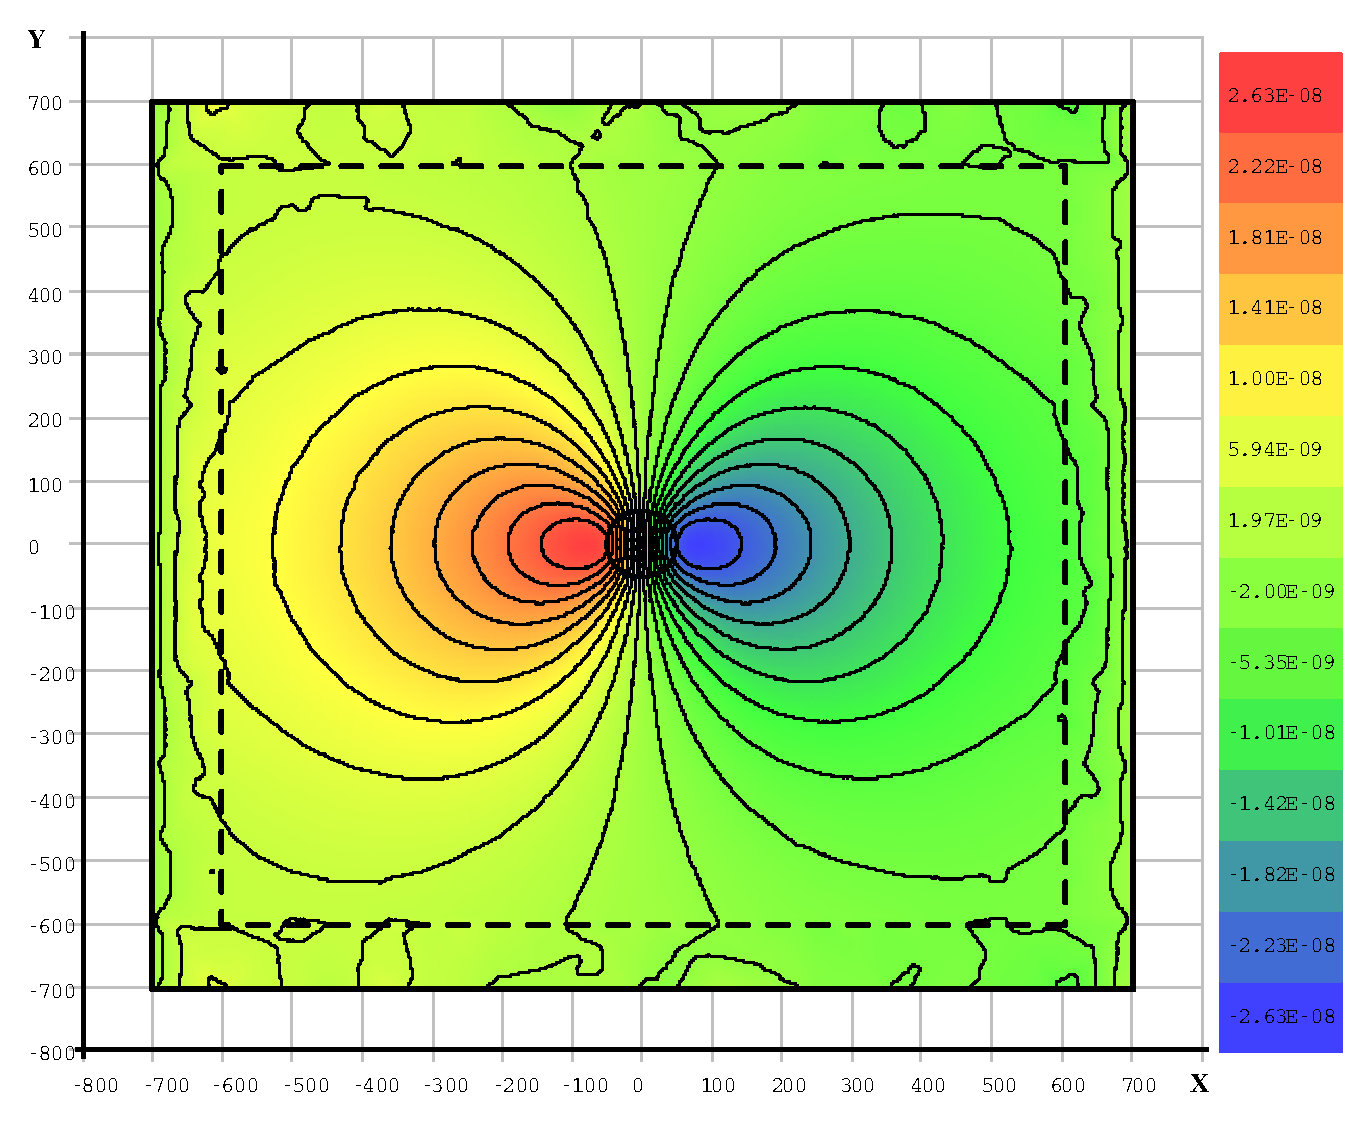
\includegraphics[scale=0.35]{research-2/field/airloop/pml/airloop_pml_z=-10_EyR.eps}\label{fig:res2:field_sca_a}}
	~~
	\subfloat[][]{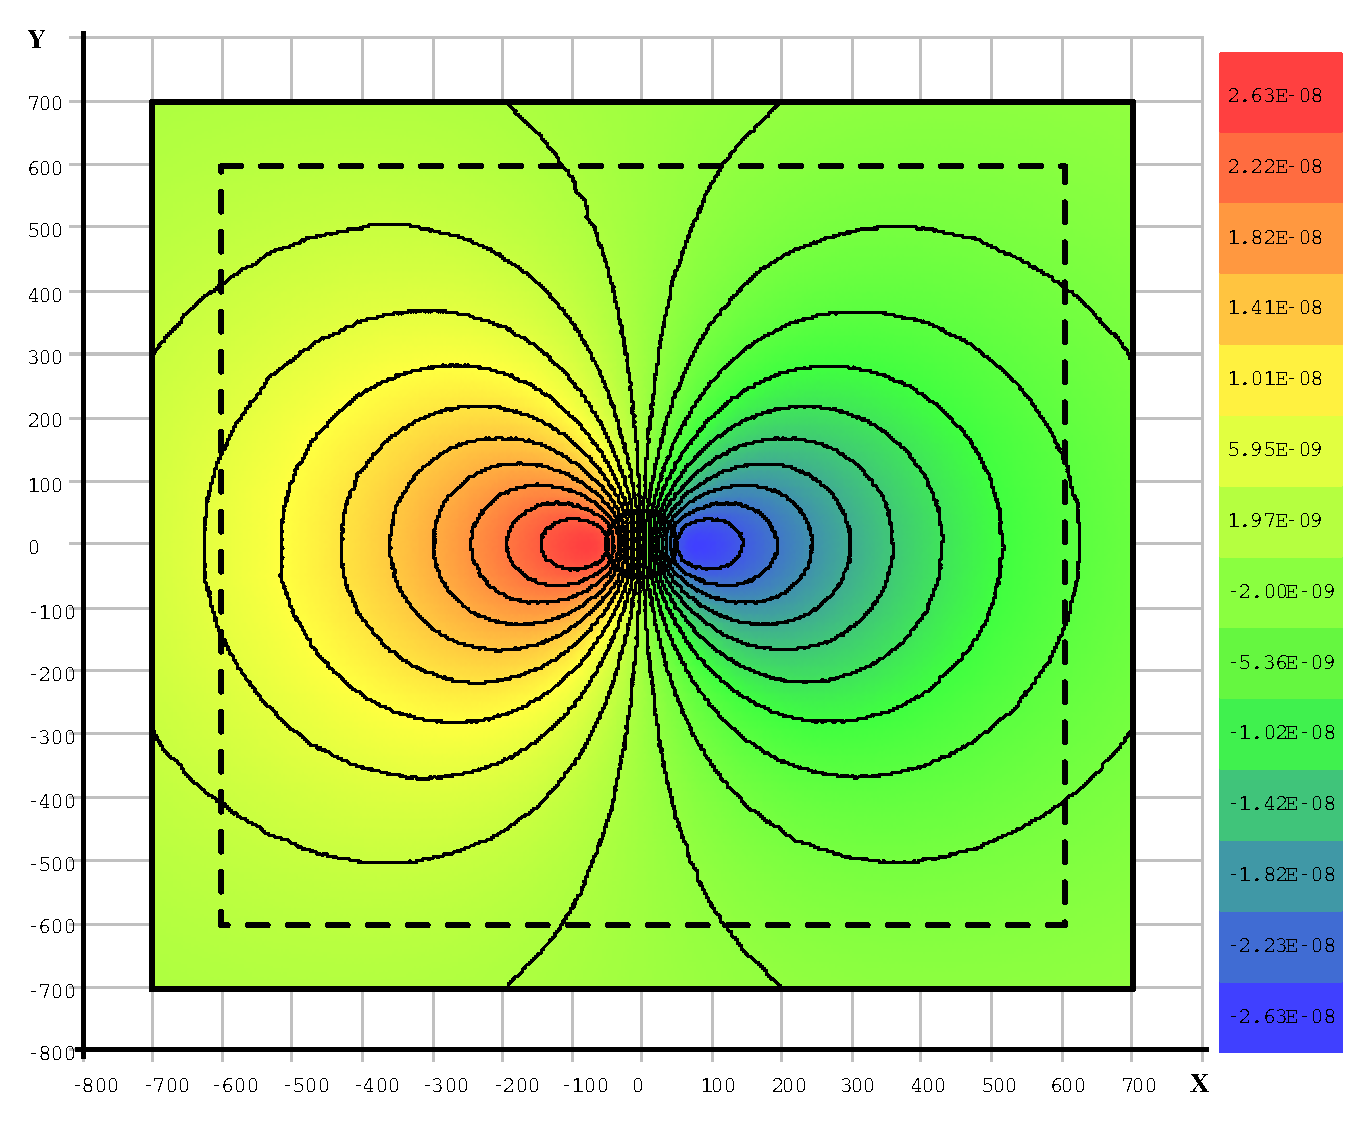
\includegraphics[scale=0.35]{research-2/field/airloop/std/airloop_std_z=-10_EyR.eps}\label{fig:res2:field_sca_b}}
	\caption{$\Re(\mathbf{E}_y)$}
	\label{fig:res2:field_sca}
\end{figure}

\vspace{-0.8cm}

\begin{figure}[H]
	\centering
	\subfloat[][]{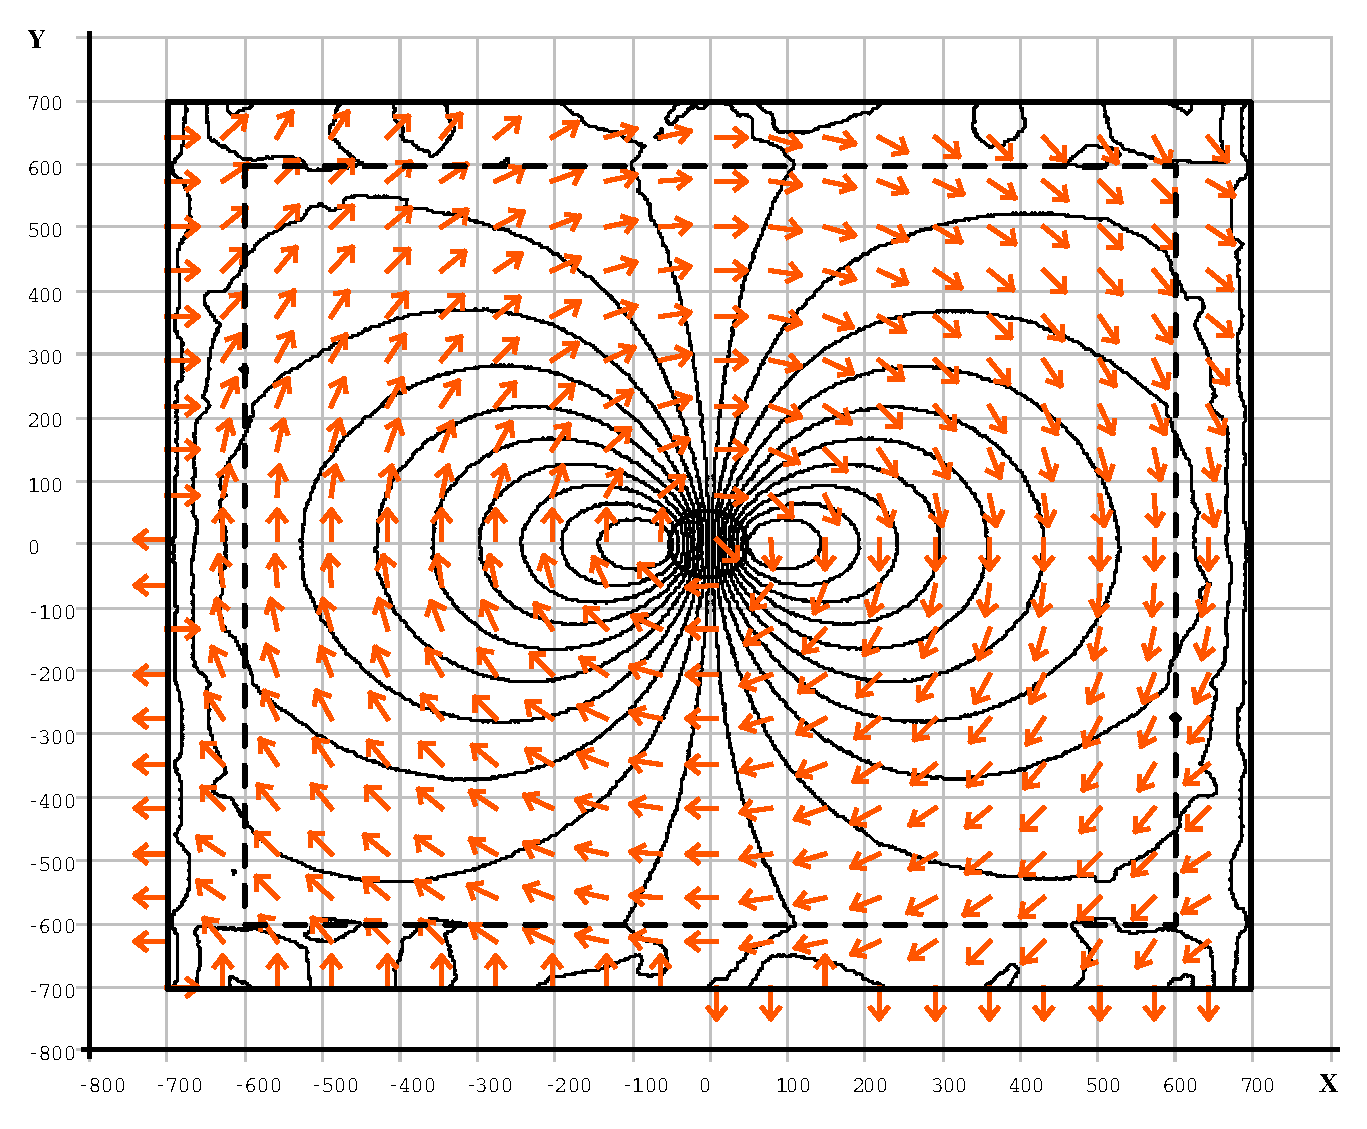
\includegraphics[scale=0.35]{research-2/field/airloop/pml/airloop_pml_z=-10_EyR_vec.eps}\label{fig:res2:field_vec_a}}
	~~
	\subfloat[][]{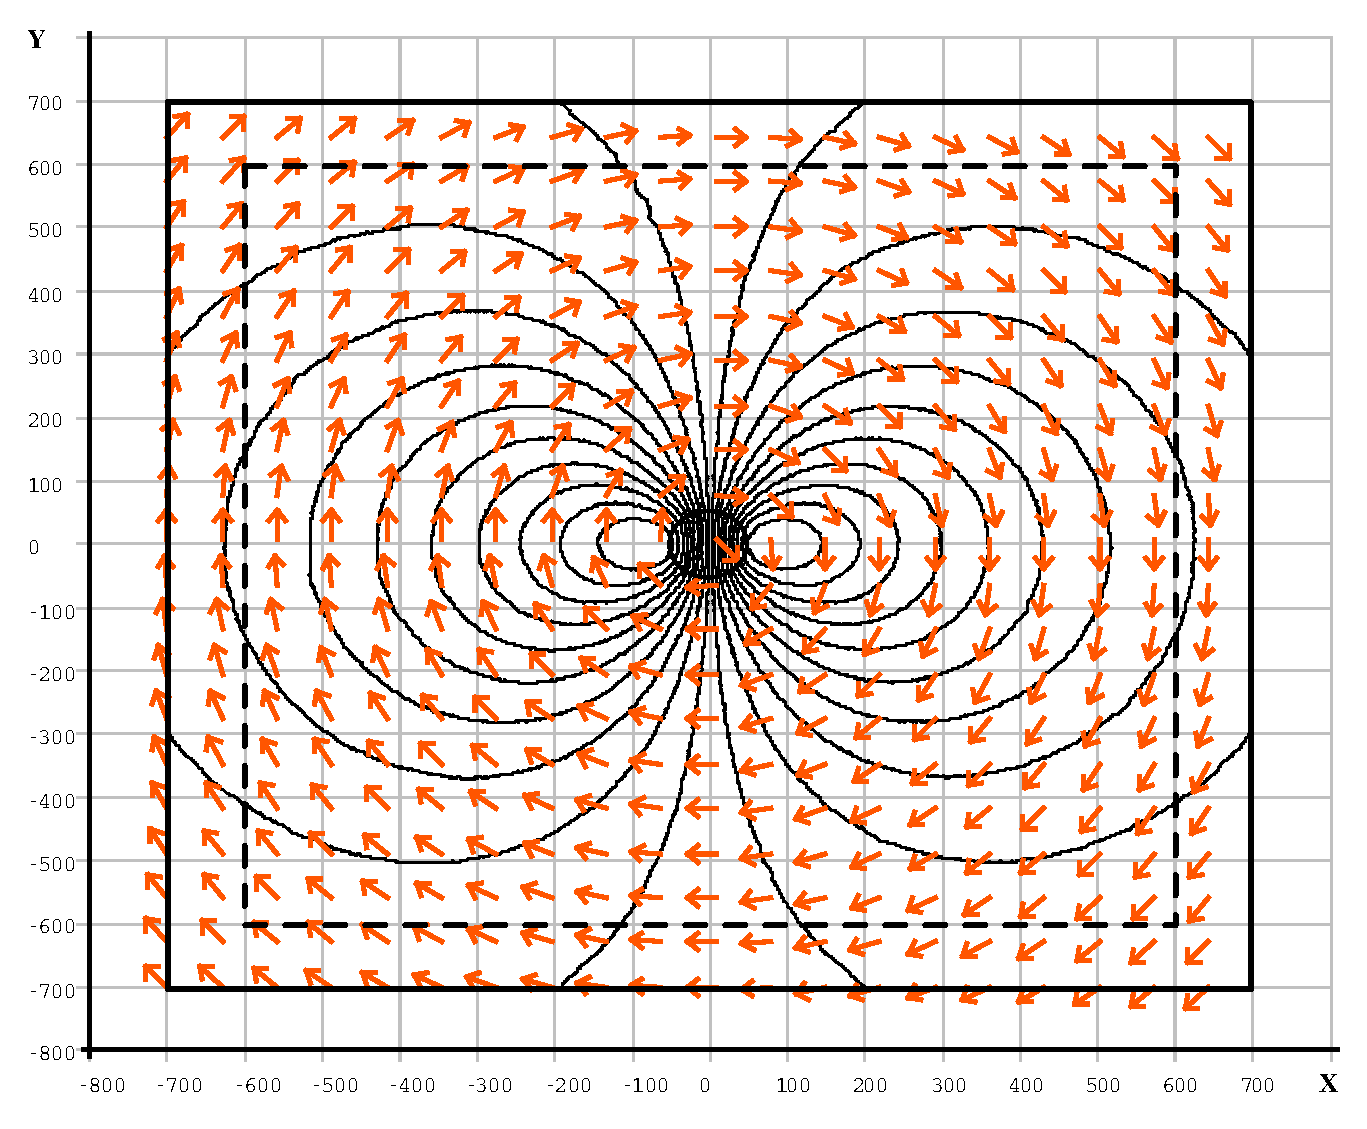
\includegraphics[scale=0.35]{research-2/field/airloop/std/airloop_std_z=-10_EyR_vec.eps}\label{fig:res2:field_vec_b}}
	\caption{изолинии $\Re(\mathbf{E}_y)$ и векторы $\left( \Re(\mathbf{E}_x) , \Re(\mathbf{E}_y) \right)^T$}
	\label{fig:res2:field_vec}
\end{figure}

\vspace{-0.8cm}

\begin{figure}[H]
	\centering
	\subfloat[][]{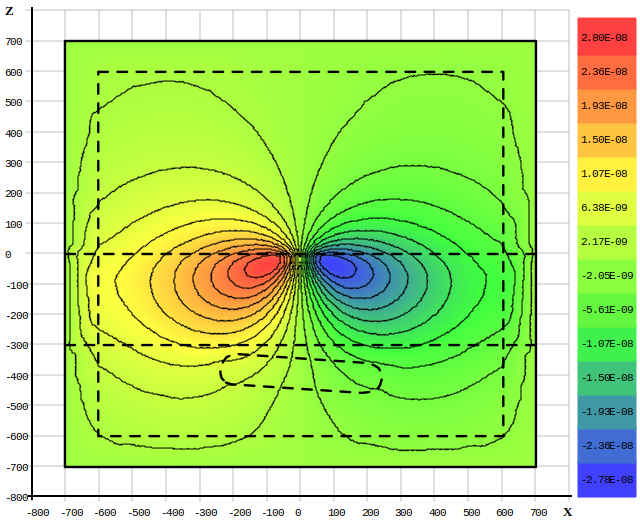
\includegraphics[scale=0.35]{research-2/field/airloop/pml/airloop_pml_y=0_EyR.eps}\label{fig:res2:field_y0_a}}
	~~
	\subfloat[][]{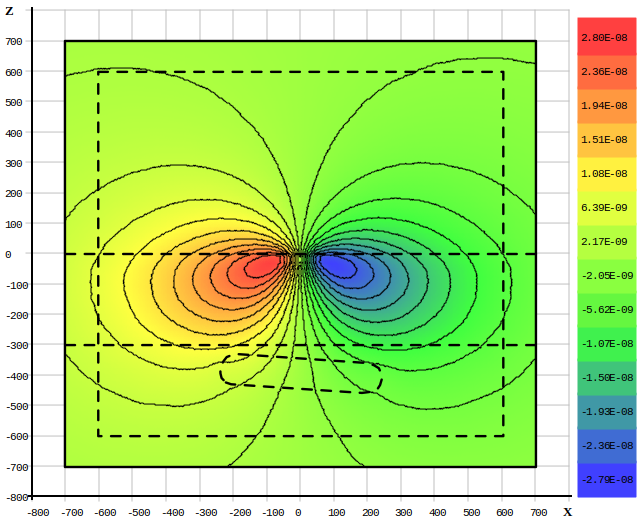
\includegraphics[scale=0.35]{research-2/field/airloop/std/airloop_std_y=0_EyR.eps}\label{fig:res2:field_y0_b}}
	\caption{$\Re(\mathbf{E}_y)$}
	\label{fig:res2:field_y0}
\end{figure}

На рисунке \ref{fig:res2:field_y0} показаны картины электрического поля в сечении плоскостью $y=0$. На рисунках \ref{fig:res2:field_y0_a} и \ref{fig:res2:field_y0_b} представлено решение с PML-слоем и решение с <<большим баком>> соответственно.


% =============================================================================

\subsubsection{Анализ целесообразности применения PML-слоя}
Наибольшее влияние на точность получаемого решения при введении PML-слоя оказывают коэффициент комплексного растяжения координат $\chi$ и $l$ -- размер области, на границе которой вводится PML-слой. При увеличении размера внутренней области ожидаемо увеличивается размер СЛАУ, поэтому этот параметр при решении реальных задач следует не варьировать, а выбрать как некоторое ограничение. Таким образом, в первую очередь стоит проводить поиск оптимального значения именно для коэффициента растяжения $\chi$. Выбор толщины PML-слоя влияет на точность решения незначительно, поэтому достаточно лишь убедиться, что она выбрана в подходящих для задачи пределах -- не слишком большой и не слишком маленькой.

В рассмотренном виде применение PML-слоя для сокращения области моделирования задач низкочастотной морской геоэлектрики незначительно уменьшает размерность СЛАУ и, в большинстве случаев, не приводит к существенному сокращению времени решения задачи. Одной из причин этого может быть то, что основное растяжение приходится на вещественные компоненты координат. Это приводит к значительной <<вытянутости>> тетраэдров внутри PML-слоя и, как следствие, сильному ухудшению свойств матрицы СЛАУ и увеличению времени решения. Параллелепипедальные конечные элементы лишены подобного недостатка, поэтому для них можно проводить комплексное растяжение в гораздо больших диапазонах. Однако, такие элементы не подходят для аппроксимации сколь-либо сложных областей. Для использования в одной сетке и тетраэдральных, и параллелепипедальных конечных элементов можно применять специальные переходные элементы~\citep{extra_elements1,extra_elements2}, либо воспользоваться неконформными методами~\citep{dg1,dg2,dg3,mortar1,mortar2}.

% =============================================================================

\clearpage
\phantomsection
\section*{Заключение}
\addcontentsline{toc}{section}{Заключение}
В работе были реализованы алгоритмы на базе векторного метода конечных элементов. Эти алгоритмы были положены в основу программного комплекса, который позволяет моделировать электромагнитные поля в областях разнообразной структуры. С помощью этого программного комплекса были решены модельные задачи морской геоэлектрики на низких частотах, проведены исследования возможности сокращения области моделирования без внесения дополнительных погрешностей.

На основании исследований были сделаны выводы, что расчеты, в которых в область моделирования не включается воздух, допустимы только при расположении источника электромагнитного поля на большой глубине, иначе, из-за неправильного учета физических процессов, происходящих в воздухе, полученное решение будет неверным.

Применение PML-слоя позволило получить достаточно точные решения, однако его применение не привело к резкому уменьшению размерности систем уравнений и, как следствие, к уменьшению времени решения. Было выдвинуто предположение, что увеличить эффективность применения PML-слоя можно с помощью применения неконформных методов, в которых конечноэлементная сетка может содержать геомитрические носители разного типа: тетраэдры и параллелепипеды.

% =============================================================================

\clearpage
\addcontentsline{toc}{section}{Список литературы}

\begin{thebibliography}{10}
% 1
\bibitem{shurina} 
Шурина, Э.П. Морская геоэлектрика -- задачи и перспективы / Э.П.~Шурина, М.И.~Эпов, А.В.~Мариенко // Тез. докл. всеросс. науч.-техн. конф. <<Научное и техническое обеспечение исследования и освоения шельфа Северного Ледовитого океана>>. -- 2010. -- 9-13~августа. -- С.~7-12.
% 2
\bibitem{gabrielsen} 
Gabrielsen, P.T. 3D CSEM for Hydrocarbon Exploration in the Barents Sea / P.T.~Gabrielsen, D.V.~Shantsev, S.~Fanavoll // 5th Saint Petersburg International Conference \& Exhibition -- Geosciences: Making the most of the Earth’s resources. -- 2012. -- 2-5~April. -- Pp.~1-5.
% 3
\bibitem{anderson}
Anderson, C. An integrated approach to marine electromagnetic surveying using a towed streamer and source / C. Anderson, J. Mattsson // First Break. -- May~2010. -- Vol.~28, Iss.~5. -- Pp.~71-75.
% 5
\bibitem{mur}
Mur G. Absorbing boundary conditions for the finite-difference approximation of the time-domain electromagnetic-field equations // Electromagnetic Compatibility, IEEE Transactions on. -- 1981. -- No.~4. -- Pp.~377-382.
% 6
\bibitem{berenger}
Berenger, J.P. A perfectly matched layer for the absorption of electromagnetic waves / J.P. Berenger // Journal of computation physics. -- 1994 -- No.~114. -- Pp.~185-200.
% 7
\bibitem{wiik_dehoop_ursin}
Wiik, T. A Discontinuous Galerkin Method for Modelling Marine Controlled Source Electromagnetic Data / T.~Wiik, M.V.~De Hoop, B.~Ursin // Proceedings of the Project Review, Geo-Mathematical Imaging Group, Purdue University, West Lafayette, IN. -- 2013 -- Vol.~1 -- P.~75-102.
% 8
\bibitem{balandin_vfem}
Баландин, М.Ю. Векторный метод конечных элементов : Учеб. пособие / М.Ю.~Баландин, Э.П.~Шурина. -- Новосибирск : Изд-во НГТУ, 2001. -- 69~с.
% 9
\bibitem{monk}
Monk P. Finite element methods for Maxwell's equations. / P.~Monk -- Oxford University Press, 2003.
% 14
\bibitem{epov}
Эпов, М.И. Параллельные конечноэлементные вычислительные схемы в задачах геоэлектрики / М.И.~Эпов, Э.П.~Шурина, Д.А.~Архипов // Вычислительные технологии. -- 2013. -- Том~18, №2. -- С.~94-112.
% 15
\bibitem{schwarzbach}
Schwarzbach C. Stability of finite element solutions to Maxwell's equations in frequency domain. / C.~Schwarzbach -- 2009.
% 16
\bibitem{hiptmair}
Hiptmair R. Multigrid method for Maxwell's equations / R.~Hiptmair // SIAM Journal on Numerical Analysis. -- 1998. -- Vol.~36. -- No.~1. -- Pp.~204-225.
% 17
\bibitem{nedelec1980}
Nédélec J.C. Mixed finite elements in $\mathbb{R}$3 / J.C.~Nédélec // Numerische Mathematik. -- 1980. -- Vol.~35. -- No.~3. -- Pp.~315-341.
% 18
\bibitem{nedelec1986}
Nédélec J.C. A new family of mixed finite elements in $\mathbb{R}$3 / J.C.~Nédélec // Numerische Mathematik. -- 1986. -- Vol.~50. -- No.~1. -- Pp.~57-81.
% 19
\bibitem{webb1993}
Webb J.P. Edge elements and what they can do for you / J.P.~Webb // Magnetics, IEEE Transactions on. -- 1993. -- Vol.~29. -- No.~2. -- Pp.~1460-1465.
% 20
\bibitem{balandin_slae}
Баландин М.Ю. Методы решения СЛАУ большой размерности: Учеб. пособие / М.Ю.~Баландин, Э.П.~Шурина. -- Новосибирск : Изд-во НГТУ, 2000. -- 70~с.
% 21
\bibitem{soloveychick}
Соловейчик, Ю.Г. Метод конечных элементов для решения скалярных и векторных задач : учеб. пособие / Ю.Г.~Соловейчик, М.Э.~Рояк, М.Г.~Персова. -- Новосибирск : Изд-во НГТУ, 2007. -- 896~с.
% 22
\bibitem{webb1999}
Webb, J.P. Hierarchal Vector Basis Functions of Arbitrary Order for Triangular and Tetrahedral Finite Elements / J.P.~Webb // IEEE transactions on antennas and propagation. -- 1999. -- Vol.~47. -- Pp.~1244-1253.
% 23
\bibitem{nechaev}
Nechaev, O.V. Multilevel iterative solver for the edge fem solution of the 3D Maxwell equation / O.V.~Nechaev, E.P.~Shurina, M.A.~Botchev // Computers and Mathematics with Applications. -- 2008. -- No.~55. -- Pp.~2346-2362.
% 24
\bibitem{mikhajlova}
Михайлова Е.И., Шурина Э.П. Математическое моделирование высокочастотного электромагнитного поля в волноводных устройствах / Е.И.~Михайлова, Э.П.~Шурина // Вестник НГУ. Серия: Математика, механика, информатика. -- 2013. -- Т.~13. -- №.~4. -- С.~102-118.
% 25
\bibitem{misovskih}
Мысовских И.П. Интерполяционные кубатурные формулы. -- Наука. Гл. ред. физ.-мат. лит., 1981.
% 26
\bibitem{zhang_integration}
Zhang L. et al. A set of symmetric quadrature rules on triangles and tetrahedra / L.~Zhang, T.~Cui, H.~Liu // J. Comput. Math. -- 2009. -- Vol.~27. -- No.~1. -- Pp.~89-96.
% 33
\bibitem{extra_elements1}
Solin P., Segeth K., Dolezel I. Higher-order finite element methods. / P.~Solin, K.~Segeth, I.~Dolezel -- CRC Press, 2003. -- 388~p.
% 34
\bibitem{extra_elements2}
Bergot M., Duruflé M. High-order optimal edge elements for pyramids, prisms and hexahedra / M.~Bergot, M.~Duruflé // Journal of Computational Physics. -- 2013. -- Vol.~232. -- No.~1. -- Pp.~189-213.
% 35
\bibitem{dg1}
Dosopoulos S., Zhao B., Lee J.F. Non-conformal and parallel discontinuous Galerkin time domain method for Maxwell’s equations: EM analysis of IC packages / S.~Dosopoulos, B.~Zhao, J.F.~Lee // Journal of Computational Physics. -- 2013. -- Vol.~238. -- Pp.~48-70.
% 36
\bibitem{dg2}
Perugia I., Schötzau D. The \textit{hp}-local discontinuous Galerkin method for low-frequency time-harmonic Maxwell equations / I.~Perugia, D.~Schötzau // Mathematics of Computation. -- 2003. -- Vol.~72. -- No.~243. -- Pp.~1179-1214.
% 37
\bibitem{dg3}
Dosopoulos S., Lee J.F. Interconnect and lumped elements modeling in interior penalty discontinuous Galerkin time-domain methods / S.~Dosopoulos, J.F.~Lee // Journal of Computational Physics. -- 2010. -- Vol.~229. -- No.~22. -- Pp.~8521-8536.
% 38
\bibitem{mortar1}
Christophe A. et al. An Overlapping Nonmatching Grid Mortar Element Method for Maxwell's Equations / A.~Christophe et al. // Magnetics, IEEE Transactions on. -- 2014. -- Vol.~50. -- Iss.~2. -- Pp.~409-412.
% 39
\bibitem{mortar2}
Gopalakrishnan J., Pasciak J.E. Multigrid for the mortar finite element method / J.~Gopalakrishnan, J.E.~Pasciak // SIAM Journal on Numerical Analysis. -- 2000. -- Vol.~37. -- No.~3. -- Pp.~1029-1052.
\end{thebibliography}

% =============================================================================

\clearpage
\phantomsection
\section*{Приложение А. Текст основного модуля программы}
\addcontentsline{toc}{section}{Приложение А. Текст основного модуля программы}
%\phantomsection
%\addcontentsline{toc}{subsection}{Файл fem.h}
%\subsection*{Файл fem.h}
\begin{singlespace}
\begin{tiny}
\begin{verbatim}
// Класс векторный МКЭ
class VFEM
{
public:
    // Конфигурация
    config_type config;

    // Ввод данных
    bool input_phys(const string & phys_filename);
    bool input_mesh(const string & gmsh_filename);
    // Процедура для сборки СЛАУ
    void make_struct();
    void make_data();
    // Запуск решения СЛАУ
    void solve();
    // Вывод данных в 3D сетке
    bool output(const string & tecplot_filename);
    // Вывод данных в 2D сетке
    bool output_slice(const string & tecplot_filename, char slice_var, double slice_val,
                      char var1, double min_var1, double max_var1, size_t num_var_1,
                      char var2, double min_var2, double max_var2, size_t num_var_2);
    // Вывод данных по линии
    bool output_line(const string & tecplot_filename, char line_var1, double line_val1,
                     char line_var2, double line_val2, char var3, double min_var3,
                     double max_var3, size_t num_var);

    // Поиск конечного элемента по точке
    finite_element * get_fe(const point & p) const;

    // Решение в точке
    cvector3 solution(const point & p) const;
    cvector3 solution(const point & p, const finite_element * fe) const;
    // Ротор решения в точке
    cvector3 rotor(const point & p) const;
    cvector3 rotor(const point & p, const finite_element * fe) const;

    // Конечные элементы (тетраэдры)
    vector<finite_element> fes;

    void calculate_diff();

    // Основная СЛАУ
    SLAE slae;
    // СЛАУ на ядре
    SLAE ker_slae;
    // СЛАУ по границе
    SLAE surf_slae;

    // Узлы
    vector<point> nodes;
    // Ребра
    set<edge> edges;
    // Грани
    set<face> faces;
    // Ребра с источниками
    vector<edge_src> edges_src;
    // Треугольники
    vector<triangle *> trs;
    // Треугольники простые
    // (не используется при config.boundary_enabled == true)
    vector<triangle_base> trs_base;
    // Треугольники полные, для первых краевых
    // (не используется при config.boundary_enabled == false)
    vector<triangle_full> trs_full;
    // Точечные источники
    vector<pair<point, cvector3> > pss;
    // Физические области
    map<phys_id, phys_area> phys;

    // Число степеней свободы
    size_t dof_num;
    // Число степеней свободы ядра
    size_t ker_dof_num;
    // Соответствие глобальных степеней свободы и по границе
    // (не используется при config.boundary_enabled == false)
    map<size_t, size_t> global_to_local;
    // Степени свободы с первыми краевыми
    // (не используется при config.boundary_enabled == true)
    set<size_t> dof_first;
    // Степени свободы с первыми краевыми у ядра
    set<size_t> ker_dof_first;
    // Восьмиричное дерево поиска
    octree<finite_element> tree;

    // Получение степеней свободы тетраэдра в глобальной матрице
    size_t get_tet_dof(const tetrahedron_base * fe, size_t i) const;
    // Получение степеней свободы тетраэдра в матрице ядра
    size_t get_tet_ker_dof(const tetrahedron_base * fe, size_t i) const;
    // Получение степеней свободы треугольника в глобальной матрице
    size_t get_tr_dof(const triangle * tr, size_t i) const;
    // Получение степеней свободы треугольника в матрице ядра
    size_t get_tr_ker_dof(const triangle * tr, size_t i) const;
    // Получение степеней свободы треугольника в матрице по границе
    size_t get_tr_surf_dof(const triangle * tr, size_t i) const;

    // Генерация портрета глобальной матрицы
    void generate_portrait();
    // Генерация портрета глобальной матрицы ядра
    void generate_ker_portrait();
    // Сборка глобальной матрицы
    void assemble_matrix();
    // Применение краевых условий
    void applying_bound();
    // Генерация портрета по границе
    void generate_surf_portrait();
    // Применение источников на ребрах
    void apply_edges_sources();
    // Применение точечных источников
    void apply_point_sources();

protected:
    // Добавление локальных матриц от одного КЭ в глобальную
    template<typename U, typename V>
    void process_fe(const U * fe, const V *);

    // Добавление ребра в множество ребер
    size_t add_edge(edge ed, set<edge> & edges_set);
    // Добавление грани в множество граней
    size_t add_face(face fc, set<face> & faces_set);

    cpoint convert_point_to_pml(const point * p, const finite_element * fefe) const;
    void input_pml();
    // Параметры PML
    phys_pml_area phys_pml;

    // Проектирование на пространство ядра
    void to_kernel_space(const complex<double> * in, complex<double> * out) const;
    // Интерполяция на полное пространство
    void to_full_space(const complex<double> * in, complex<double> * out) const;
    // Скалярное произведение
    double dot_prod_self(const complex<double> * a) const;
    // Умножение матрицы с полного пространства на вектор
    void mul_matrix(const complex<double> * f, complex<double> * x) const;
    // Подсчет невязки
    void calc_residual(const complex<double> * x0, complex<double> * p) const;
};

void VFEM::generate_portrait()
{
    cout << "Generating portrait ..." << endl;

    set<size_t> * portrait = new set<size_t> [dof_num];
    for(size_t k = 0; k < fes.size(); k++)
    {
        show_progress("step 1", k, fes.size());

        array_t<size_t> dof(config.basis.tet_bf_num);
        for(size_t i = 0; i < config.basis.tet_bf_num; i++)
            dof[i] = get_tet_dof(&fes[k], i);

        for(size_t i = 0; i < config.basis.tet_bf_num; i++)
        {
            size_t a = dof[i];
            for(size_t j = 0; j < i; j++)
            {
                size_t b = dof[j];
                if(b > a)
                    portrait[b].insert(a);
                else
                    portrait[a].insert(b);
            }
        }
    }

    size_t gg_size = 0;
    for(size_t i = 0; i < dof_num; i++)
        gg_size += portrait[i].size();

    slae.alloc_all(dof_num, gg_size);

    slae.ig[0] = 0;
    slae.ig[1] = 0;
    size_t tmp = 0;
    for(size_t i = 0; i < dof_num; i++)
    {
        show_progress("step 2", i, dof_num);

        for(set<size_t>::iterator j = portrait[i].begin(); j != portrait[i].end(); ++j)
        {
            slae.jg[tmp] = *j;
            tmp++;
        }
        slae.ig[i + 1] = slae.ig[i] + portrait[i].size();

        portrait[i].clear();
    }

    delete [] portrait;
}

void VFEM::generate_ker_portrait()
{
    cout << "Generating kernel portrait ..." << endl;

    set<size_t> * portrait = new set<size_t> [ker_dof_num];
    for(size_t k = 0; k < fes.size(); k++)
    {
        show_progress("step 1", k, fes.size());

        array_t<size_t> ker_dof(config.basis.tet_ker_bf_num);
        for(size_t i = 0; i < config.basis.tet_ker_bf_num; i++)
            ker_dof[i] = get_tet_ker_dof(&fes[k], i);

        for(size_t i = 0; i < config.basis.tet_ker_bf_num; i++)
        {
            size_t a = ker_dof[i];
            for(size_t j = 0; j < i; j++)
            {
                size_t b = ker_dof[j];
                if(b > a)
                    portrait[b].insert(a);
                else
                    portrait[a].insert(b);
            }
        }
    }

    size_t gg_size = 0;
    for(size_t i = 0; i < ker_dof_num; i++)
        gg_size += portrait[i].size();

    ker_slae.alloc_all(ker_dof_num, gg_size);

    ker_slae.ig[0] = 0;
    ker_slae.ig[1] = 0;
    size_t tmp = 0;
    for(size_t i = 0; i < ker_dof_num; i++)
    {
        show_progress("step 2", i, ker_dof_num);

        for(set<size_t>::iterator j = portrait[i].begin(); j != portrait[i].end(); ++j)
        {
            ker_slae.jg[tmp] = *j;
            tmp++;
        }
        ker_slae.ig[i + 1] = ker_slae.ig[i] + portrait[i].size();

        portrait[i].clear();
    }

    delete [] portrait;
}

void VFEM::generate_surf_portrait()
{
    cout << "Generaing surface portrait ..." << endl;

    size_t dof_surf_num = global_to_local.size();
    set<size_t> * portrait = new set<size_t> [dof_surf_num];
    for(size_t k = 0; k < trs.size(); k++)
    {
        show_progress("step 1", k, trs.size());

        array_t<size_t> dof_surf(config.basis.tr_bf_num);
        for(size_t i = 0; i < config.basis.tr_bf_num; i++)
            dof_surf[i] = get_tr_surf_dof(trs[k], i);

        if(trs[k]->phys->type_of_bounds == 1)
        {
            for(size_t i = 0; i < config.basis.tr_bf_num; i++)
            {
                size_t a = dof_surf[i];
                for(size_t j = 0; j < i; j++)
                {
                    size_t b = dof_surf[j];
                    if(b > a)
                        portrait[b].insert(a);
                    else
                        portrait[a].insert(b);
                }
            }
        }
    }

    size_t gg_size = 0;
    for(size_t i = 0; i < dof_surf_num; i++)
        gg_size += portrait[i].size();

    surf_slae.alloc_all(dof_surf_num, gg_size);

    surf_slae.ig[0] = 0;
    surf_slae.ig[1] = 0;
    size_t tmp = 0;
    for(size_t i = 0; i < dof_surf_num; i++)
    {
        show_progress("step 2", i, dof_surf_num);

        for(set<size_t>::iterator j = portrait[i].begin(); j != portrait[i].end(); ++j)
        {
            surf_slae.jg[tmp] = *j;
            tmp++;
        }
        surf_slae.ig[i + 1] = surf_slae.ig[i] + portrait[i].size();

        portrait[i].clear();
    }

    delete [] portrait;
}

// Добавление локальных матриц от одного КЭ в глобальную
template<typename U, typename V>
void VFEM::process_fe(const U * curr_fe, const V *)
{
    // Получение физических параметров для заданного КЭ
    phys_area ph = curr_fe->get_phys_area();
    complex<double> k2(- ph.epsilon * ph.omega * ph.omega, ph.omega * ph.sigma);

    // Инициализация параметров вычислителей для правой части
    pair<const config_type *, array_t<evaluator<complex<double> > *, 3> >
            params_object(& config, array_t<evaluator<complex<double> > *, 3>());
    if(config.right_enabled)
    {
        map<size_t, array_t<evaluator<complex<double> >, 3> >::iterator
                it = config.right.values.find(ph.gmsh_num);
        if(it != config.right.values.end())
            for(size_t i = 0; i < 3; i++)
                params_object.second[i] = &(it->second[i]);
        else
            for(size_t i = 0; i < 3; i++)
            {
                evaluator<complex<double> > * ev_curr = &(config.right.default_value[i]);
                params_object.second[i] = ev_curr;
                ev_curr->set_var("epsilon", ph.epsilon);
                ev_curr->set_var("sigma", ph.sigma);
                ev_curr->set_var("mu", ph.mu);
                ev_curr->set_var("J0", ph.J0);
                ev_curr->set_var("k2", k2);
            }
    }

    // Получение степеней свободы
    array_t<size_t> dof(config.basis.tet_bf_num);
    for(size_t i = 0; i < config.basis.tet_bf_num; i++)
        dof[i] = get_tet_dof(curr_fe, i);

    // Получение локальных матриц и правой части
    V matrix_G = curr_fe->G();
    V matrix_M = curr_fe->M();
    array_t<complex<double> > array_rp = curr_fe->rp(func_rp, &params_object);

    // Основная матрица
    for(size_t i = 0; i < config.basis.tet_bf_num; i++)
    {
        complex<double> add;
        size_t i_num = dof[i];
        for(size_t j = 0; j < i; j++)
        {
            size_t j_num = dof[j];
            add = matrix_G[i][j] / ph.mu + matrix_M[i][j] * k2;
            slae.add(i_num, j_num, add);
        }
        add = matrix_G[i][i] / ph.mu + matrix_M[i][i] * k2;
        slae.di[i_num] += add;
        add = array_rp[i];
        slae.rp[i_num] += add;
    }

    // Матрица ядра
    if(config.v_cycle_enabled)
    {
        array_t<size_t> ker_dof(config.basis.tet_ker_bf_num);
        for(size_t i = 0; i < config.basis.tet_ker_bf_num; i++)
            ker_dof[i] = get_tet_ker_dof(curr_fe, i);

        V matrix_K = curr_fe->K();
        for(size_t i = 0; i < config.basis.tet_ker_bf_num; i++)
        {
            size_t i_num = ker_dof[i];
            for(size_t j = 0; j < i; j++)
                ker_slae.add(i_num, ker_dof[j], matrix_K[i][j] * k2);
            ker_slae.di[i_num] += matrix_K[i][i] * k2;
        }
    }
}

void VFEM::assemble_matrix()
{
    cout << "Assembling matrix ..." << endl;

    cout << " > Assembling matrix ..." << endl;
    // Cборка основной матрицы
    for(size_t k = 0; k < fes.size(); k++)
    {
        show_progress("", k, fes.size());
        if(!is_pml(fes[k].barycenter, &fes[k], &phys_pml))
            process_fe(fes[k].to_std(), (matrix_t<double> *)NULL);
        else
            process_fe(&fes[k], (l_matrix *)NULL);
    }
}

void VFEM::applying_bound()
{
    cout << " > Applying first bound ..." << endl;

    if(config.boundary_enabled)
    {

        // Решение СЛАУ по границе
        if(global_to_local.size() > 0)
        {
            for(size_t k = 0; k < trs.size(); k++)
            {
                show_progress("building matrix", k, trs.size());

                phys_area ph = trs[k]->get_phys_area();
                if(ph.type_of_bounds == 1)
                {
                    // Получение физических параметров для текущего треугольника границы
                    complex<double> k2(- ph.epsilon * ph.omega * ph.omega, ph.omega * ph.sigma);

                    // Инициализация параметров вычислителей для первого краевого
                    pair<const config_type *, array_t<evaluator<complex<double> > *, 3> >
                            params_object(& config, array_t<evaluator<complex<double> > *, 3>());
                    map<size_t, array_t<evaluator<complex<double> >, 3> >::iterator
                            it = config.boundary.values.find(ph.gmsh_num);
                    if(it != config.boundary.values.end())
                        for(size_t i = 0; i < 3; i++)
                            params_object.second[i] = &(it->second[i]);
                    else
                        for(size_t i = 0; i < 3; i++)
                        {
                            evaluator<complex<double> > * ev_curr = &(config.boundary.default_value[i]);
                            params_object.second[i] = ev_curr;
                            ev_curr->set_var("epsilon", ph.epsilon);
                            ev_curr->set_var("sigma", ph.sigma);
                            ev_curr->set_var("mu", ph.mu);
                            ev_curr->set_var("J0", ph.J0);
                            ev_curr->set_var("k2", k2);
                        }

                    // Получение степеней свободы
                    array_t<size_t> dof_surf(config.basis.tr_bf_num);
                    for(size_t i = 0; i < config.basis.tr_bf_num; i++)
                        dof_surf[i] = get_tr_surf_dof(trs[k], i);

                    // Получение локальных матриц и правой части
                    matrix_t<double> M_surf = trs[k]->M();
                    array_t<complex<double> > b_surf = trs[k]->rp(func_b1, &params_object);

                    // Добавляем полученное в матрицу с краевыми
                    for(size_t i = 0; i < config.basis.tr_bf_num; i++)
                    {
                        for(size_t j = 0; j < i; j++)
                            surf_slae.add(dof_surf[i], dof_surf[j], M_surf[i][j]);
                        surf_slae.di[dof_surf[i]] += M_surf[i][i];
                        surf_slae.rp[dof_surf[i]] += b_surf[i];
                    }
                }
            }
            surf_slae.solve(config.eps_slae_bound, config.max_iter);
        }

        // Учет первых краевых
        for(size_t k = 0; k < slae.n; k++) 	  // Пробегаем по всей матрице
        {
            show_progress("applying", k, slae.n);

            map<size_t, size_t>::iterator g2l_k = global_to_local.find(k);
            if(g2l_k != global_to_local.end())
            {
                complex<double> val = surf_slae.x[g2l_k->second];
                slae.rp[k] = val;
                slae.di[k] = 1.0;
                slae.x[k] = val; // Начальное приближение сразу знаем

                for(size_t i = slae.ig[k]; i < slae.ig[k + 1]; i++)
                {
                    if(global_to_local.find(slae.jg[i]) == global_to_local.end())
                        slae.rp[slae.jg[i]] -= slae.gg[i] * val;
                    slae.gg[i] = 0.0;
                }
            }
            else
            {
                for(size_t i = slae.ig[k]; i < slae.ig[k + 1]; i++)
                {
                    if(global_to_local.find(slae.jg[i]) != global_to_local.end())
                    {
                        complex<double> val = surf_slae.x[global_to_local[slae.jg[i]]];
                        slae.rp[k] -= slae.gg[i] * val;
                        slae.gg[i] = 0.0;
                    }
                }
            }
        }

    }
    else
    {

        for(size_t k = 0; k < slae.n; k++) 	  // Пробегаем по всей матрице
        {
            show_progress("", k, slae.n);

            if(dof_first.find(k) != dof_first.end())
            {
                slae.rp[k] = 0.0;
                slae.di[k] = 1.0;

                for(size_t i = slae.ig[k]; i < slae.ig[k + 1]; i++)
                    slae.gg[i] = 0.0;
            }
            else
            {
                for(size_t i = slae.ig[k]; i < slae.ig[k + 1]; i++)
                {
                    if(dof_first.find(slae.jg[i]) != dof_first.end())
                        slae.gg[i] = 0.0;
                }
            }
        }

    }

    if(config.v_cycle_enabled)
    {
        // Первые краевые для матрицы ядра
        for(size_t k = 0; k < ker_slae.n; k++)
        {
            // Пробегаем по всей матрице
            if(ker_dof_first.find(k) != ker_dof_first.end())
            {
                ker_slae.di[k] = 1.0;
                for(size_t i = ker_slae.ig[k]; i < ker_slae.ig[k + 1]; i++)
                    ker_slae.gg[i] = 0.0;
            }
            else
            {
                for(size_t i = ker_slae.ig[k]; i < ker_slae.ig[k + 1]; i++)
                {
                    if(ker_dof_first.find(ker_slae.jg[i]) != ker_dof_first.end())
                        ker_slae.gg[i] = 0.0;
                }
            }
        }
    }
}

void VFEM::apply_edges_sources()
{
    cout << " > Applying edges sources ..." << endl;
    for(size_t k = 0; k < edges_src.size(); k++)
    {
        show_progress("", k, edges_src.size());
        size_t pos = edges_src[k].num; // Заносим только в роторные функции!
        slae.rp[pos] += complex<double>(0.0, -1.0) * edges_src[k].phys->J0 * edges_src[k].phys->omega * edges_src[k].direction;
    }
}

finite_element * VFEM::get_fe(const point & p) const
{
    finite_element * fe = NULL;
    fe = tree.find(p.x, p.y, p.z);
    if(!fe)
        cout << "Warning: Point " << p << " is outside area!" << endl;
    return fe;
}

cvector3 VFEM::solution(const point & p) const
{
    return solution(p, get_fe(p));
}

cvector3 VFEM::solution(const point & p, const finite_element * fe) const
{
    cvector3 result;
    if(fe)
    {
        for(size_t i = 0; i < config.basis.tet_bf_num; i++)
            result = result + slae.x[get_tet_dof(fe, i)] * fe->w(i, p);
    }
    return result;
}

cvector3 VFEM::rotor(const point & p) const
{
    return rotor(p, get_fe(p));
}

cvector3 VFEM::rotor(const point & p, const finite_element * fe) const
{
    cvector3 result;
    if(fe)
    {
        for(size_t i = 0; i < config.basis.tet_bf_num; i++)
            result = result + slae.x[get_tet_dof(fe, i)] * fe->rotw(i, p);
    }
    return result;
}

void VFEM::make_struct()
{
    if(config.boundary_enabled && global_to_local.size() > 0)
        generate_surf_portrait();
    generate_portrait();
    if(config.v_cycle_enabled)
        generate_ker_portrait();
}

void VFEM::make_data()
{
    assemble_matrix();
    apply_edges_sources();
    applying_bound();
}

\end{verbatim}
\end{tiny}
\end{singlespace}

% =============================================================================

\end{document}
